\chapter{Graph Databases}
A graph is a structure that not only can represent data but also connections between them; in particular, links between data items are explicitly represented in graphs.

\section{Graphs and Graph Structures}
Graphs structure data into a set of data objects and a set of links between these objects. The \textit{data objects} are the \textbf{nodes} (vertices) and \textit{links} are the \textbf{edges} (arcs).

\begin{tcolorbox}
Graphs can store information in the nodes as well as on the edges.
\end{tcolorbox}

In a social network the \textbf{nodes} of a graph can store \textit{information on people} and \textbf{edges} can store their \textit{acquaintance} or express \textit{sympathy} or \textit{antipathy}.

Or in a geographic information systems \textbf{nodes} store information on \textit{geographical locations} like cities and \textbf{edges} store for example the \textit{distances} between the locations

\begin{figure}
     \centering
     \begin{subfigure}[b]{0.45\textwidth}
         \centering
         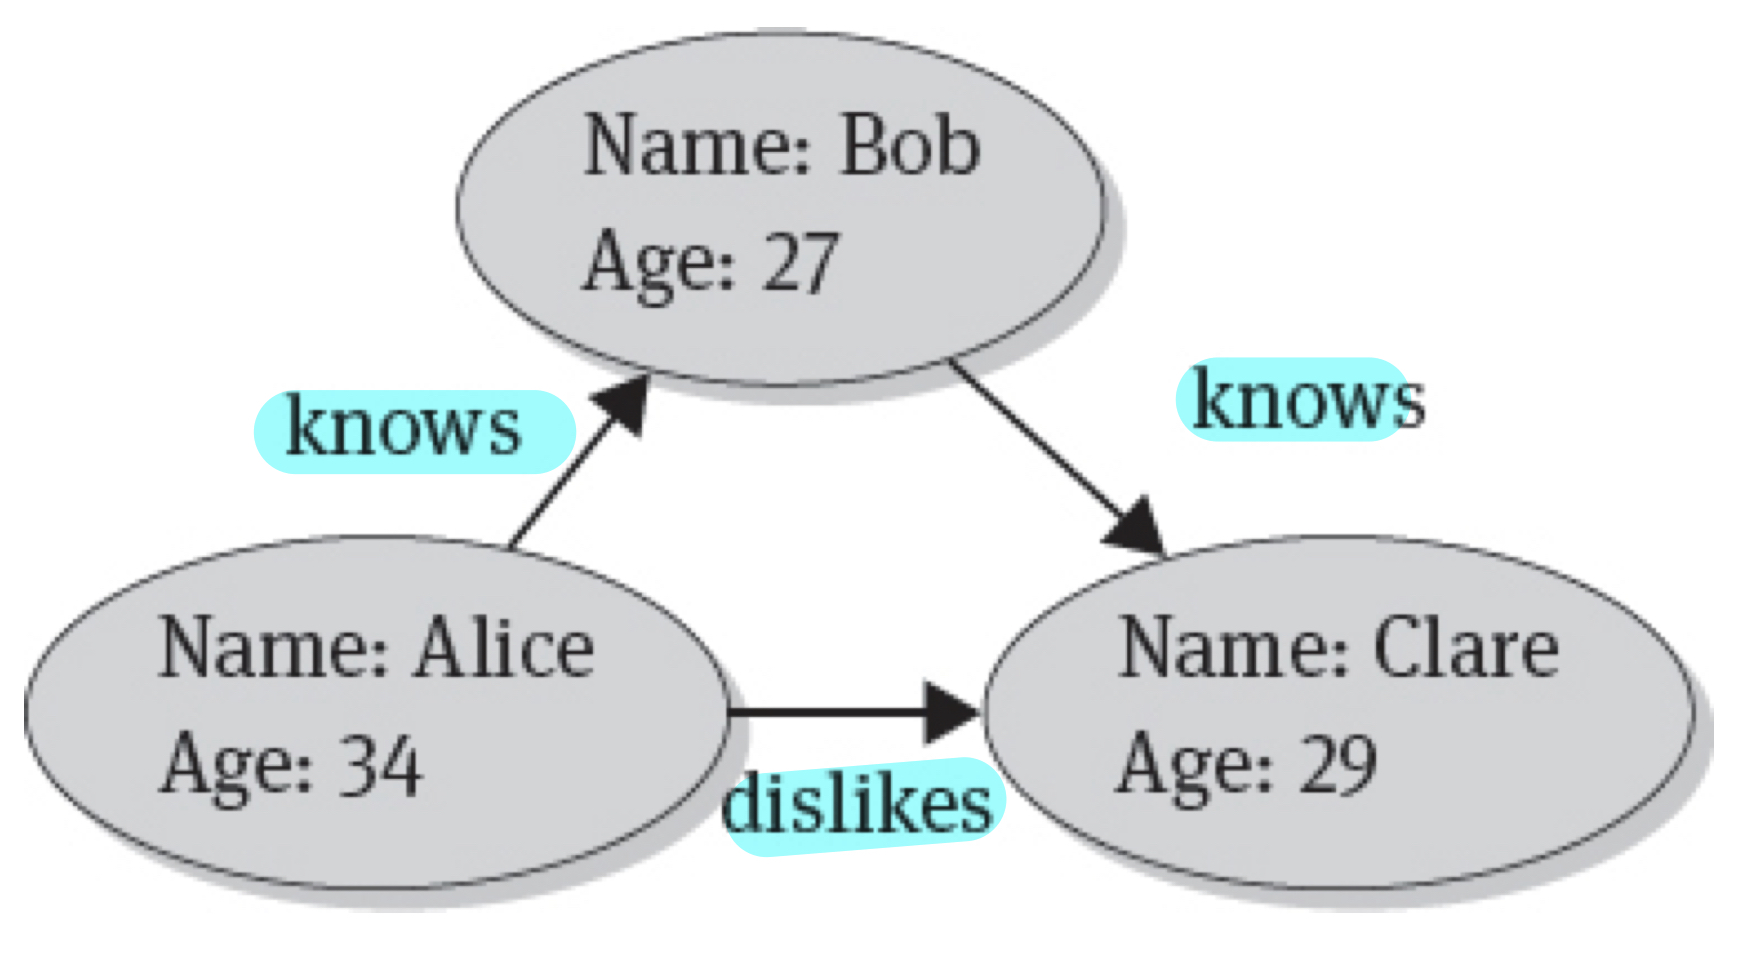
\includegraphics[width=\textwidth]{images/AdvancedDataManagment/graph_databases/social_network_example.jpeg}
         \caption{A social network as a graph}
     \end{subfigure}
     \hfill
     \begin{subfigure}[b]{0.45\textwidth}
         \centering
         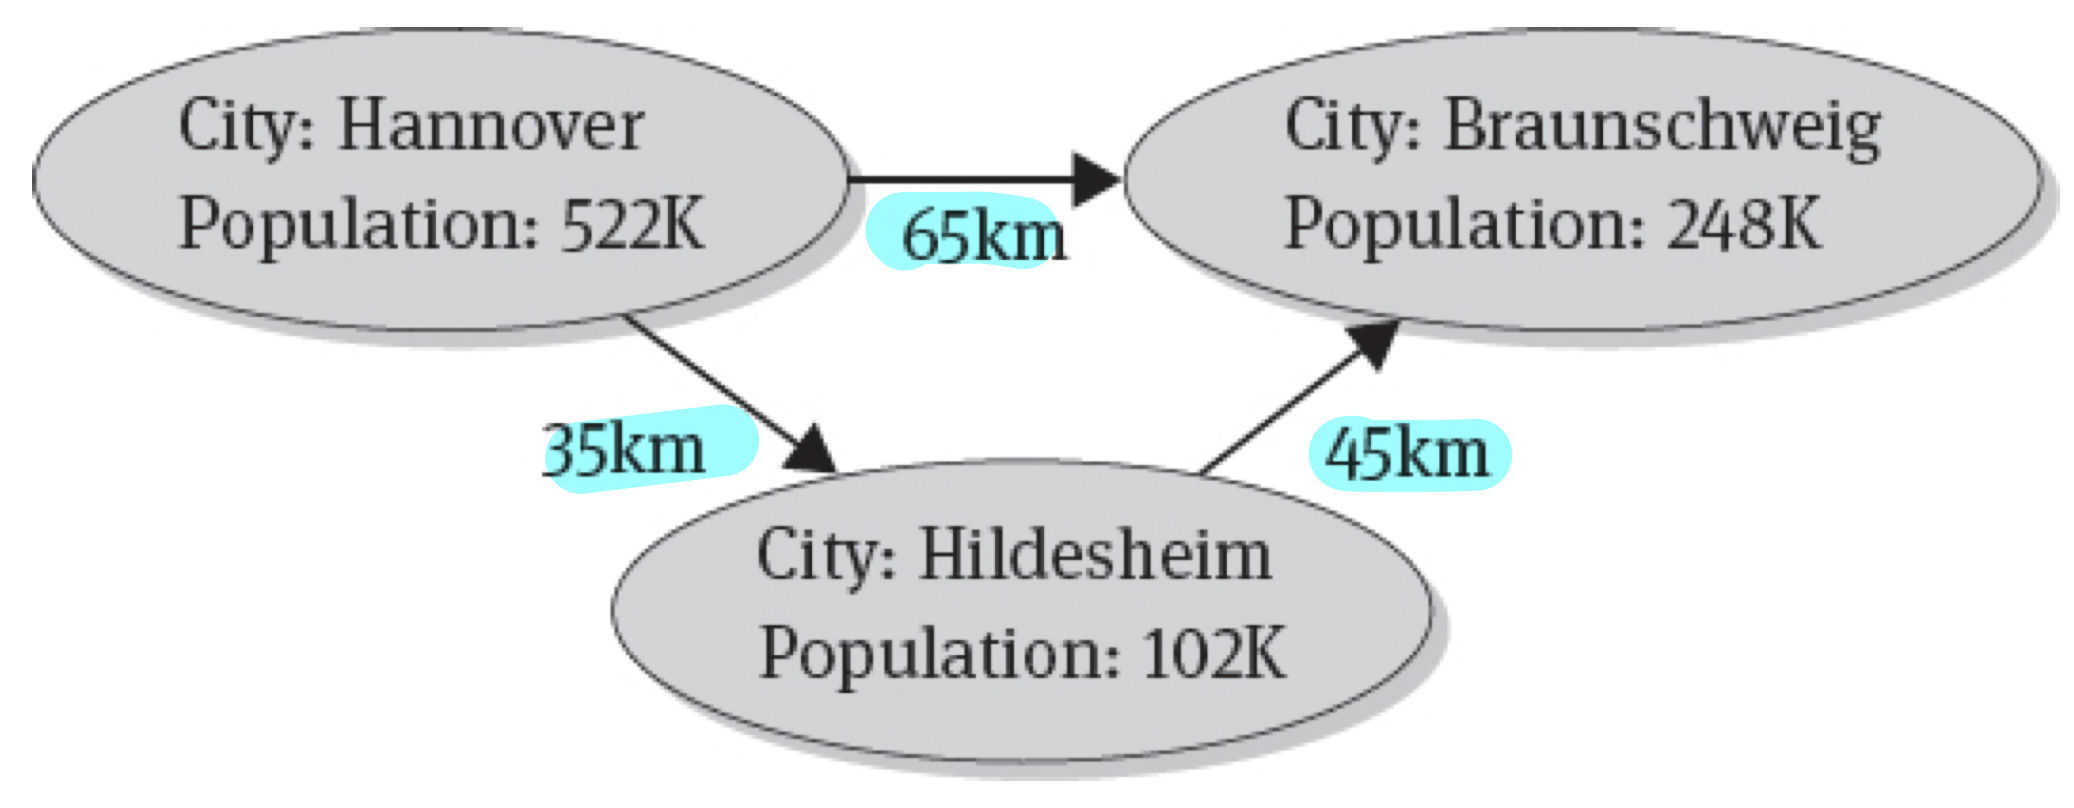
\includegraphics[width=\textwidth]{images/AdvancedDataManagment/graph_databases/geographical_example.jpeg}
         \caption{Geographical data as a graph}
     \end{subfigure}
\end{figure}

\subsection{A Glimpse on Graph Theory}
Mathematically speaking a graph \(G = (V, E)\) consists on a set of nodes \(V\) and a set of edges \(E\).
\begin{itemize}
    \item The edge set \(E\) is a set of pairs of nodes and represents vertices that are connected by the edge
    \item The edge can be \textit{directed} or \textit{undirected}:
    \begin{itemize}
        \item In a \textit{directed} edge the pair of nodes is ordered where the first node is the \textbf{source} node of the edge and the last node is the \textbf{target} node
        \item In the \textit{undirected} case, order of the pair of nodes does not matter 
    \end{itemize}
\end{itemize}
Moreover, a graph is called \textit{multigraph} if it has a pair of nodes that is connected by more than one edge. Now we have a look on a short summary on the graph types:

\begin{itemize}
    \item \textbf{Simple undirected graph:}
    \begin{figure}[!h]
        \centering
        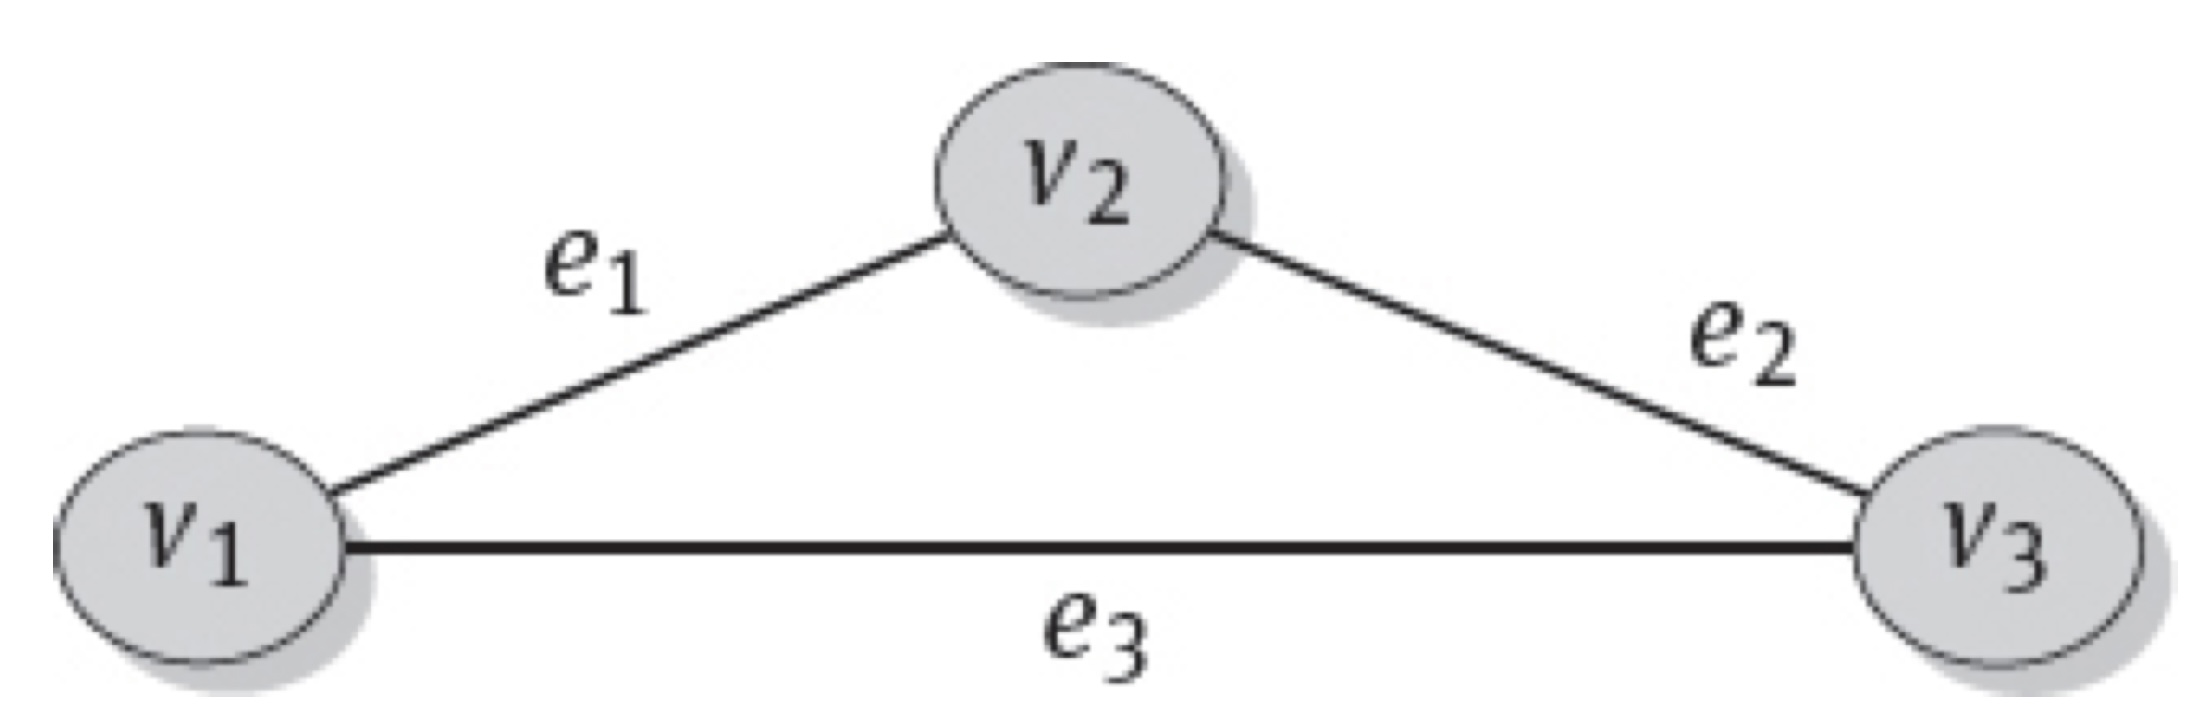
\includegraphics[width=0.35\linewidth]{images/AdvancedDataManagment/graph_databases/simple_undirected_graph.jpeg}
    \end{figure}
    
    \item \textbf{Simple directed graph:}
    \begin{figure}[!h]
        \centering
        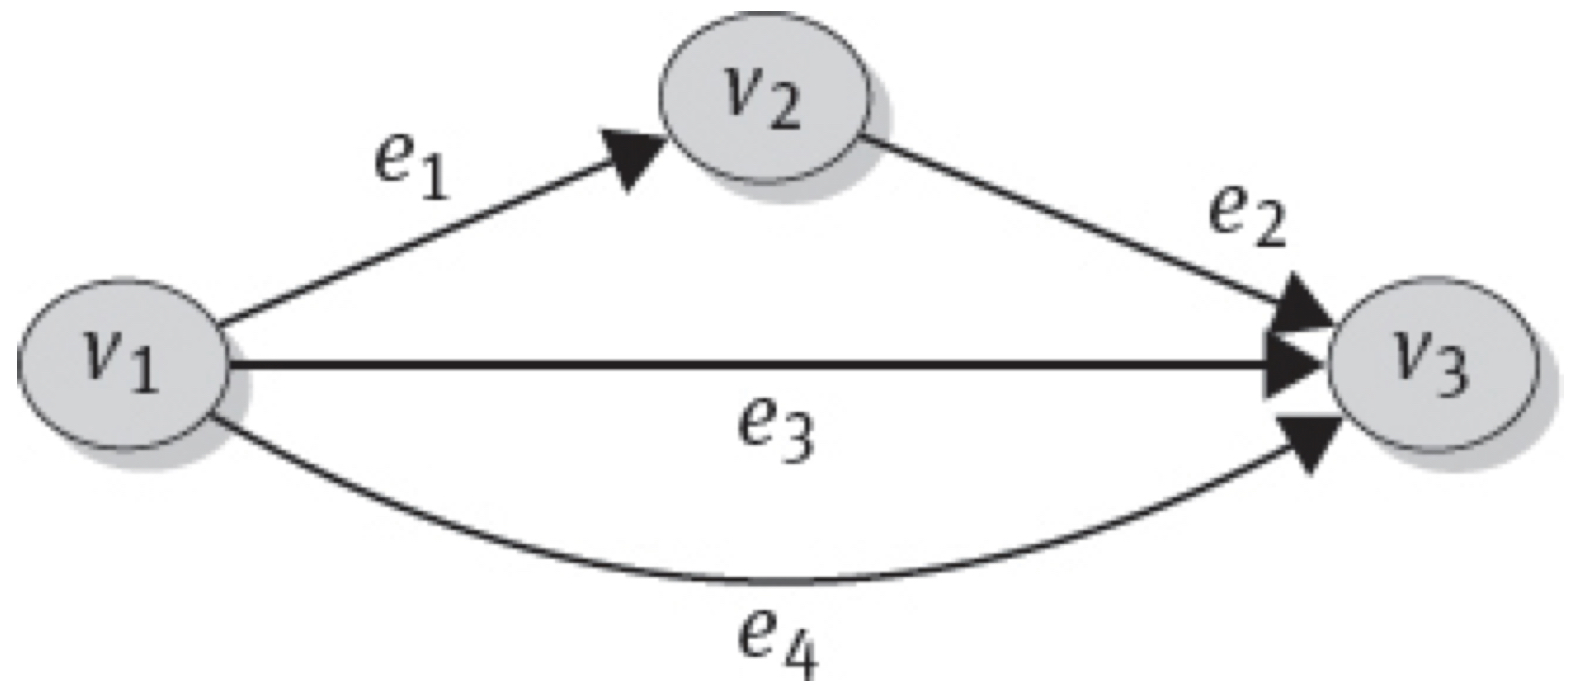
\includegraphics[width=0.35\linewidth]{images/AdvancedDataManagment/graph_databases/directed_multigraph.jpeg}
    \end{figure}
    
    \item \textbf{Undirected Multigraph:}
    \begin{figure}[!h]
        \centering
        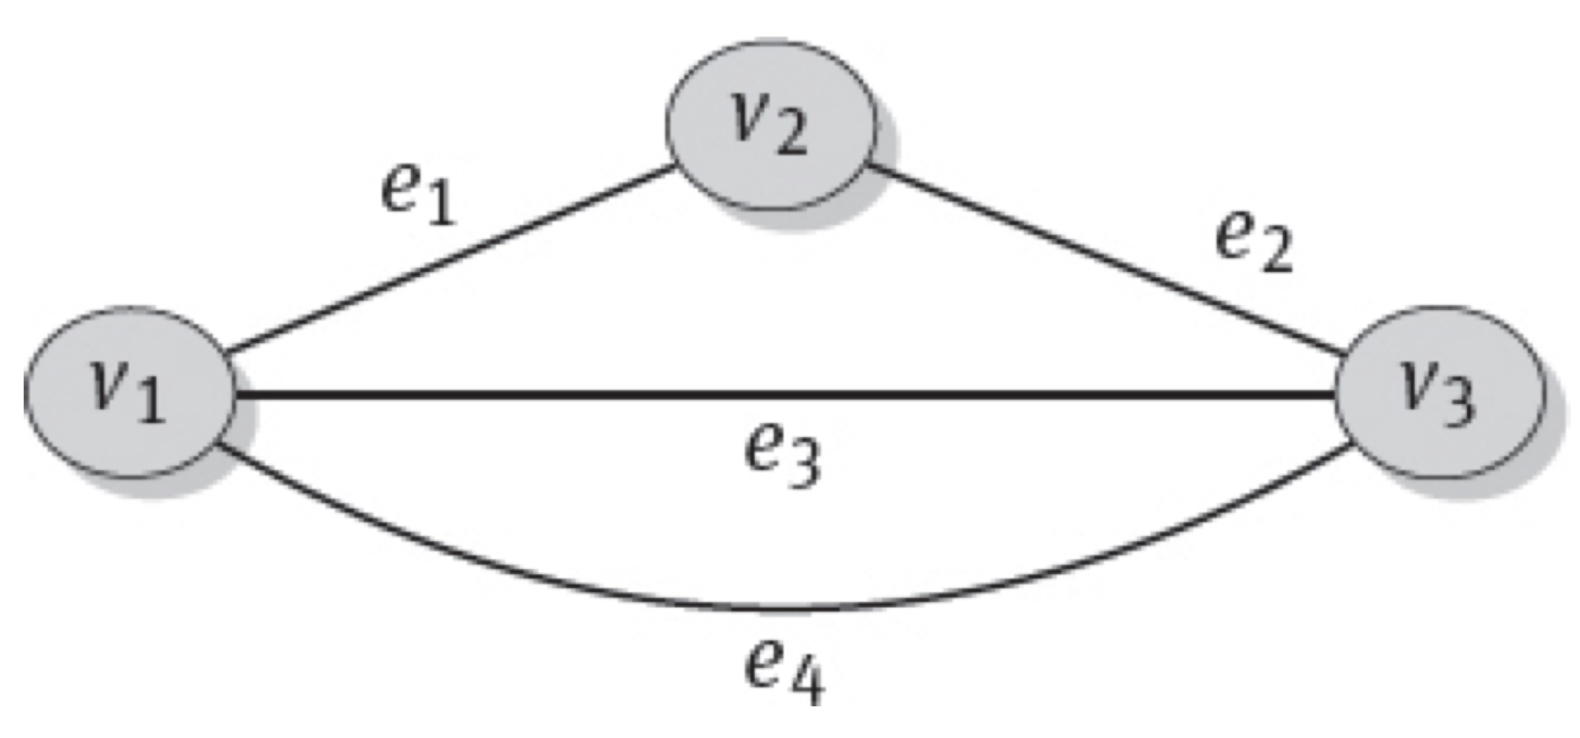
\includegraphics[width=0.35\linewidth]{images/AdvancedDataManagment/graph_databases/undirected_multigraph.jpeg}
    \end{figure}
    
    \item \textbf{Directed Multigraph:}
    \begin{figure}[!h]
        \centering
        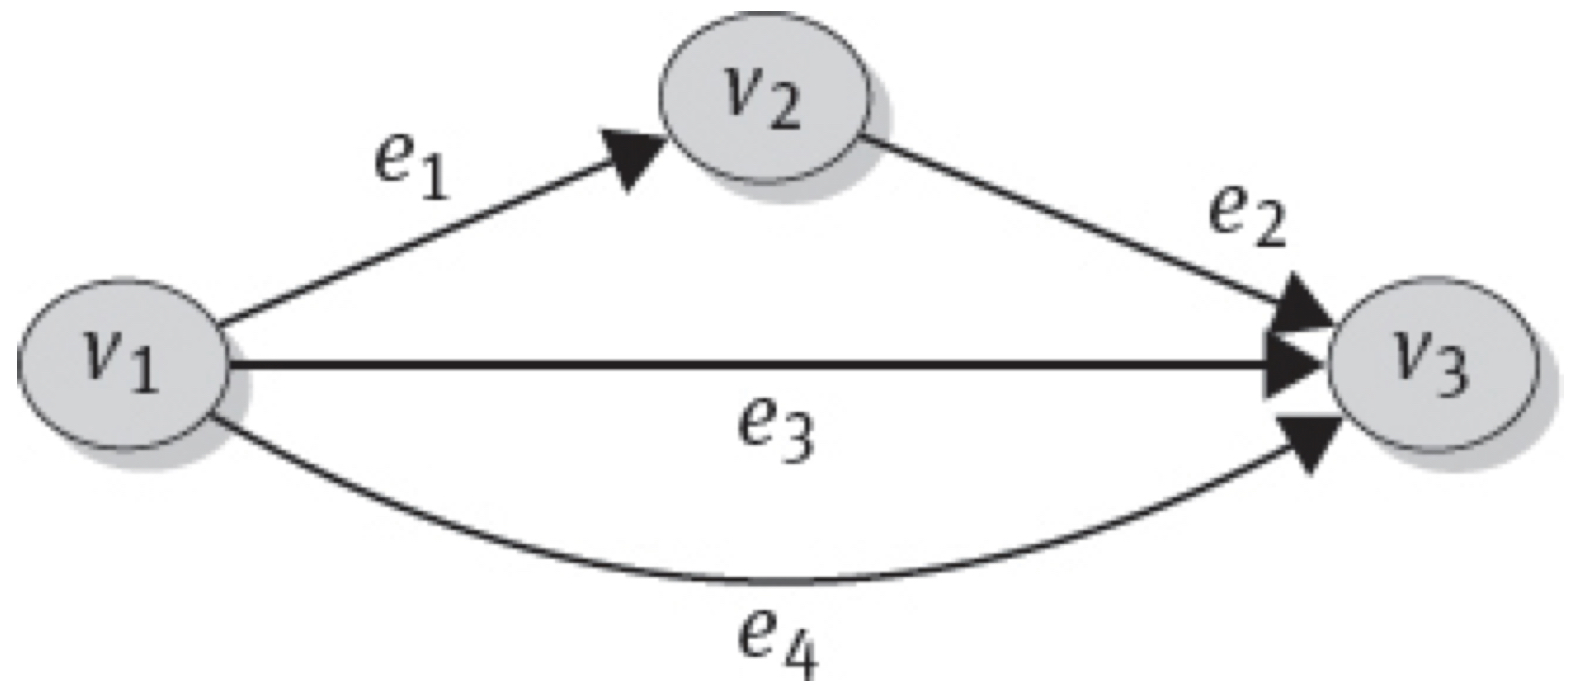
\includegraphics[width=0.35\linewidth]{images/AdvancedDataManagment/graph_databases/directed_multigraph.jpeg}
    \end{figure}
    
    \item \textbf{Weighted graphs:}
    \begin{figure}[!h]
        \centering
        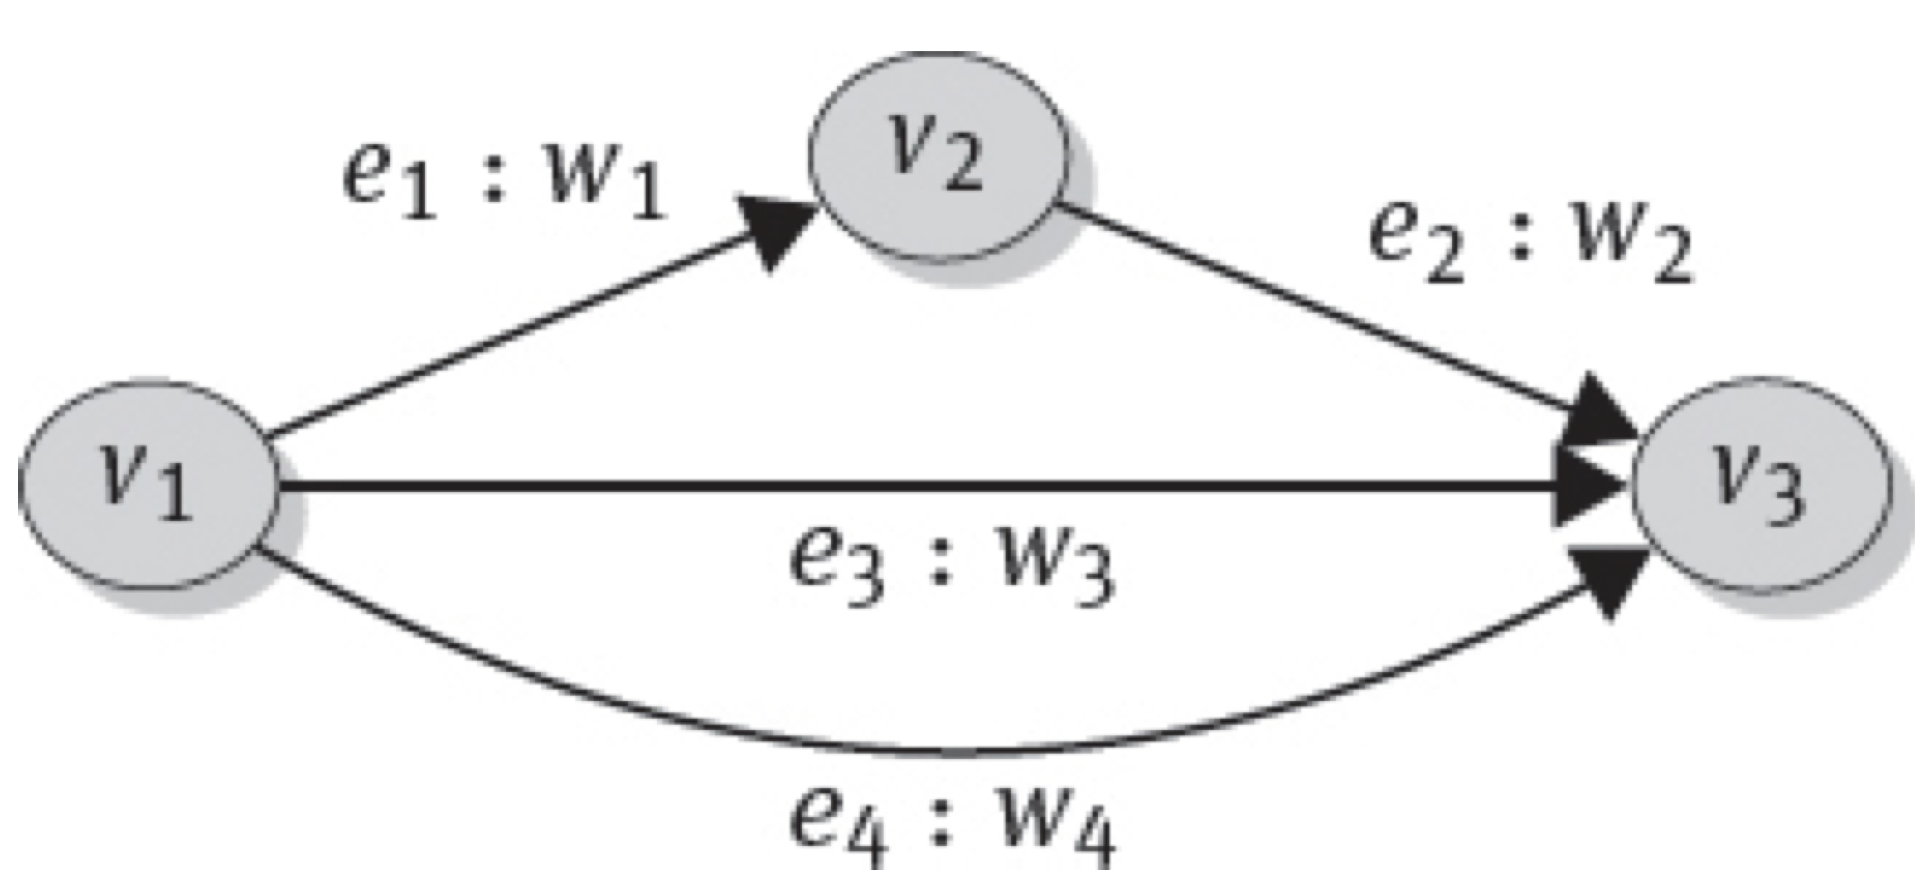
\includegraphics[width=0.35\linewidth]{images/AdvancedDataManagment/graph_databases/weighted_graph.jpeg}
    \end{figure}
\end{itemize}

\subsection{Graph Traversal and Graph Problems}
\begin{itemize}
    \item A connection between to nodes consisting of intermediary nodes and the edges between them is called a \textbf{path}
    \item A path where starting node and end node are the same is called a \textbf{cycle}
    \item A \textbf{traversal} is a sort of navigation from a starting node to a specific destination nodes towards adjacent nodes. It could be:
    \begin{itemize}
        \item \textit{full} visiting each and every node in a graph
        \item \textit{partial} in which navigation may be restricted by a certain depth of paths to be followed
    \end{itemize}
\end{itemize}
When traversing a graph, restrictions may be applied that have come to known as \textbf{graph problems}:
\begin{itemize}
    \item \textbf{Eulerian Path:} a path that visits each edge exactly once;
    \item \textbf{Eulerian Cycle:} a cycle that visits each edge exactly once;
    \item \textbf{Hamiltonian Path:} a path that visits each vertex exactly once
    \item \textbf{Hamiltonian Cycle:} a cycle that visits each vertex exactly once
    \item \textbf{Spanning Tree:} a subset of the edge set V that forms a tree and visits each node of the tree
\end{itemize}

\section{Graph Data Structures}
When computing with graphs, the information on nodes and their connecting edges has to be represented and stored in an appropriate data structure. Two important terms in this field are \textbf{adjacency} and \textbf{incidence}
\begin{tcolorbox}
Two nodes are \textbf{adjacent} if they are neighbors (that is, there is an edge between them)
\end{tcolorbox}

\begin{tcolorbox}
An edge is \textbf{incident} to a node, if it is connected to the node. Moreover if the edge is \textit{directed}:
\begin{itemize}
    \item It is \textbf{positively incident} to its \textit{source} node
    \item And \textbf{negatively incident} to its \textit{target} node
\end{itemize}
A node is incident to an edge, if it is connected to the edge.
\end{tcolorbox}

\subsection{Edge List}
The graph can be stored according to the mathematical definition as a set of nodes \(V\) and a set (or list) of edges \(E\). Edges could be represented as:
\begin{itemize}
    \item \textit{A set of sets} for \textbf{undirected graphs}
    \item \textit{A multiset set} for \textbf{multigraphs}
\end{itemize}
We can compute the classical operation:
\begin{itemize}
    \item \textbf{Addition} of an edge or nodes in which we simply add the element in the respective set
    \item \textbf{Deletion} by simply deleting the removed node or edge from the respective set
    \item \textbf{Search} the edge set performs well when one wants to retrieve all edges of the graph at once
\end{itemize}
However, the edge list representation is ineffcient in most use cases, like: looking for one particular edge or getting all neighbors of a given node requires \textit{iterating over the entire edge list}

\subsection{Adjacency Matrix}
\begin{itemize}
    \item For cardinality \(|V| = n\) the adjacent matrix is \(n \times n\) matrix
    \item Rows and columns denoted by \(v_1,...,v_n\)
    \item \textbf{Simple undirected graphs}
    \begin{itemize}
        \item If between \(v_i\) and \(v_j\) there is an edge we put a \(1\) in the corresponding cells \((v_i, v_j)\) and \((v_j, v_i)\) since \textit{symmetry}
        \item In case of \textit{loops} \(v_i, v_i\) we write \(2\) in the diagonal cell  \(v_i, v_i\)
        
        \begin{figure}[!h]
        \centering
        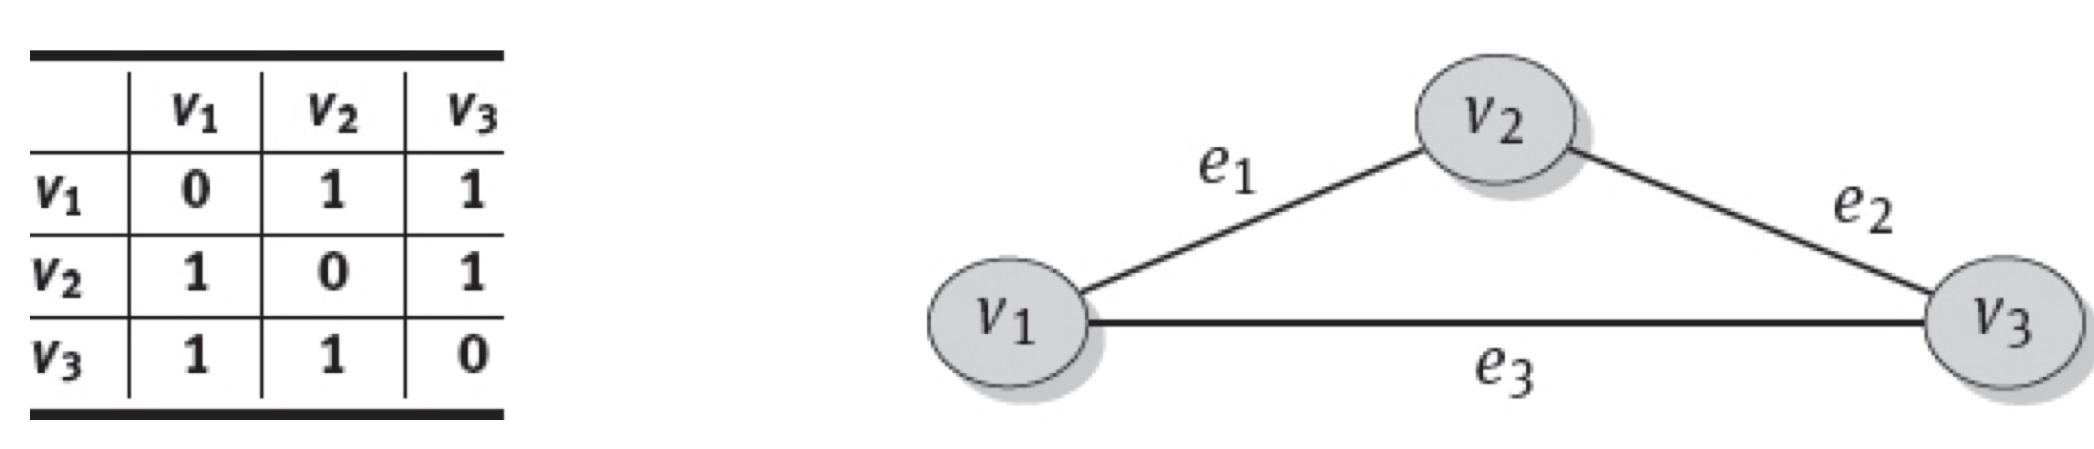
\includegraphics[width=0.7\linewidth]{images/AdvancedDataManagment/graph_databases/adj_matrix_simple_undirected.jpeg}
        \end{figure}
        
    \end{itemize}
    \item \textbf{Simple directed graph}
    \begin{itemize}
        \item If between \(v_i\) and \(v_j\) there is an edge we put a \(1\) in the corresponding cell \((v_i, v_j)\) since \textit{asymmetry}
        \item In case of \textit{loops} \(v_i, v_i\) we write \(1\) in the diagonal cell \(v_i, v_i\)
    
        \begin{figure}[!h]
        \centering
        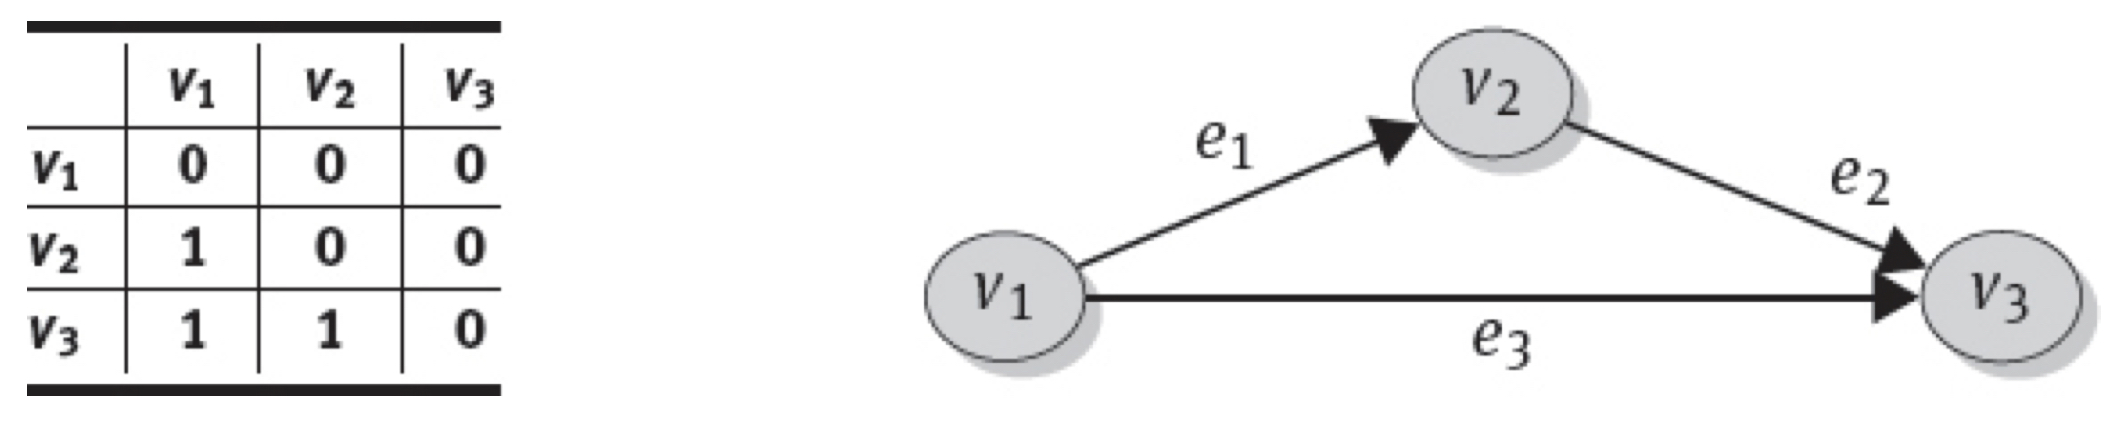
\includegraphics[width=0.7\linewidth]{images/AdvancedDataManagment/graph_databases/adj_matrix_simple_directed.jpeg}
        \end{figure}
        
    \end{itemize}
    \item \textbf{Undirected multigraph}
    \begin{itemize}
        \item If there are \(k\) edges between \(v_i\) and \(v_j\) we put a \(k\) in the corresponding cells \((v_i, v_j)\) and \((v_j, v_i)\) since \textit{symmetry}
        \item In case of \(k\) \textit{loops} \(v_i, v_i\) we write \(2 \cdot k\) in the diagonal cell \(v_i, v_i\)
    
        \begin{figure}[!h]
        \centering
        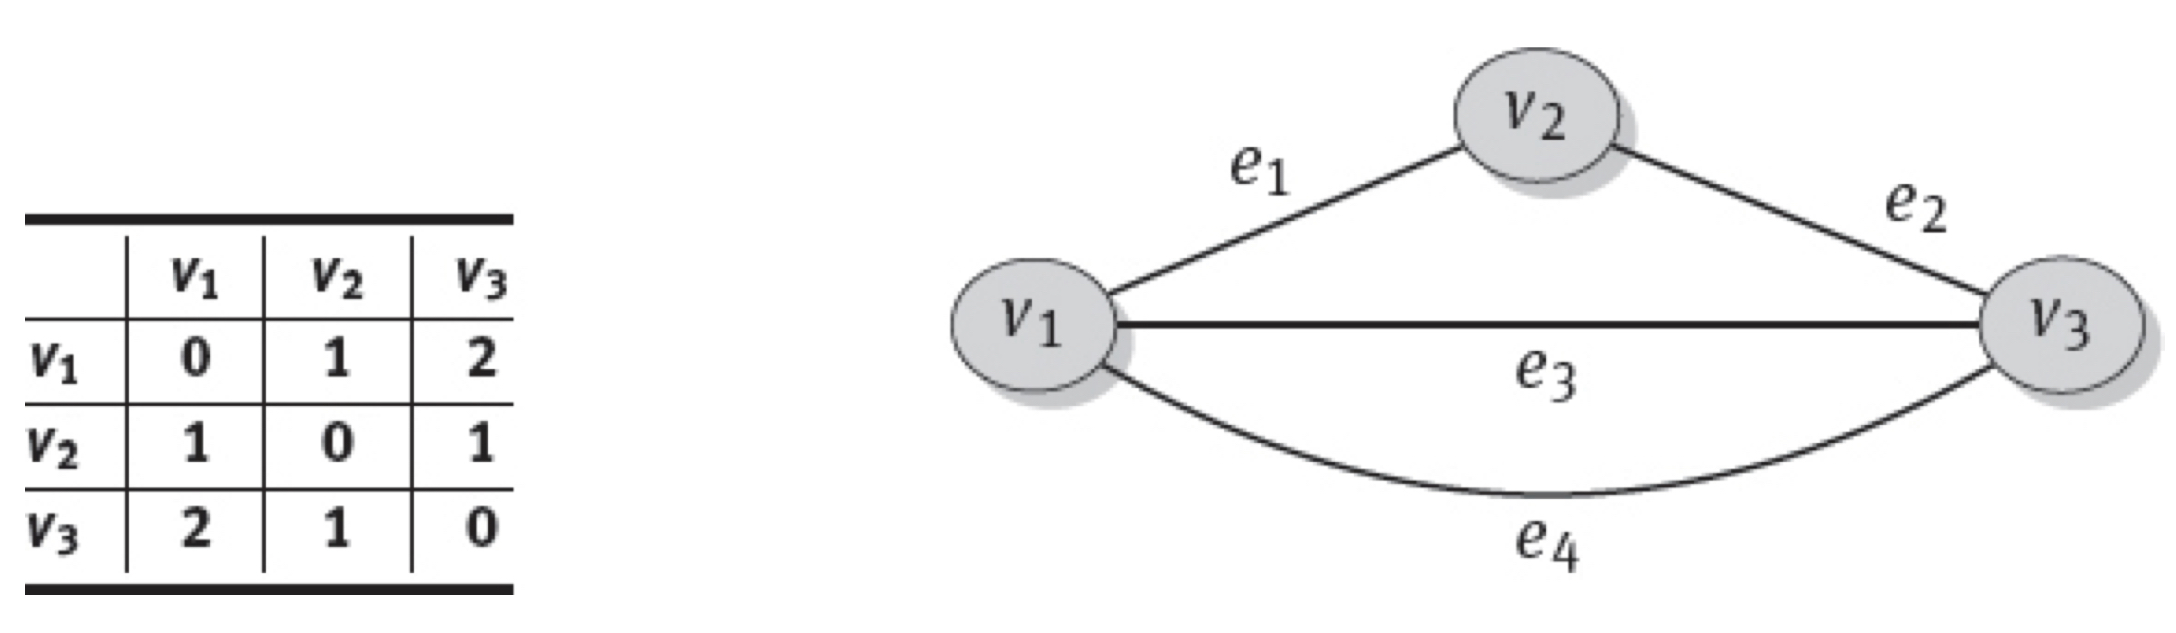
\includegraphics[width=0.7\linewidth]{images/AdvancedDataManagment/graph_databases/adj_matrix_multi_undirected.jpeg}
        \end{figure}
        
    \end{itemize}
    \item \textbf{Directed multigraph}
    \begin{itemize}
        \item If there are \(k\) edges between \(v_i\) and \(v_j\) we put a \(k\) in the corresponding cell \((v_i, v_j)\) since \textit{asymmetry}
        \item In case of \(k\) \textit{loops} \(v_i, v_i\) we write \(k\) in the diagonal cell \(v_i, v_i\)
    
        \begin{figure}[!h]
        \centering
        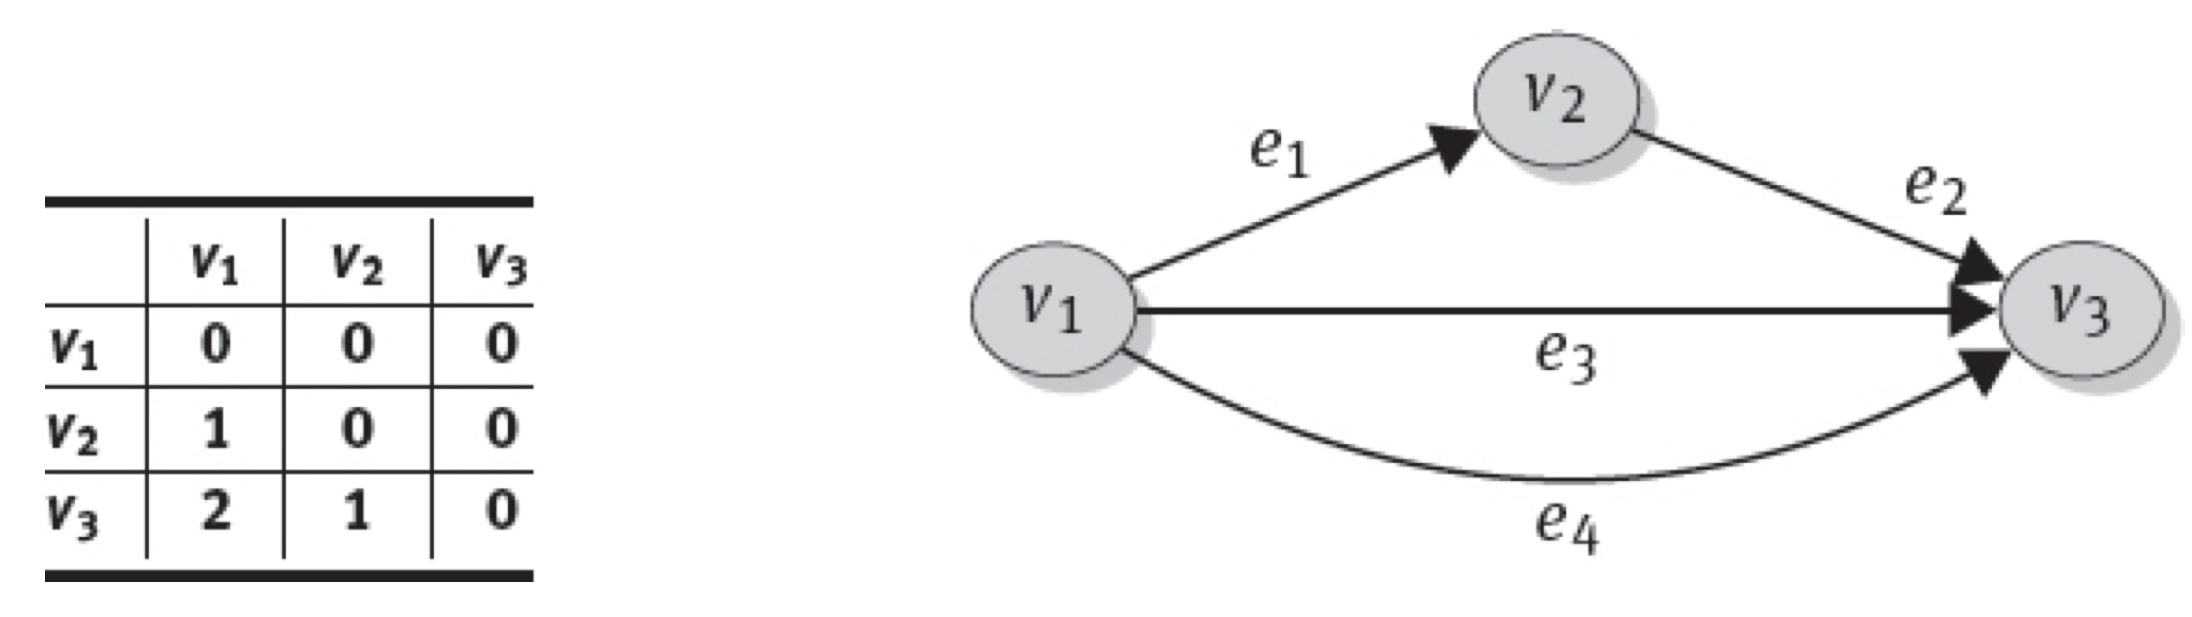
\includegraphics[width=0.7\linewidth]{images/AdvancedDataManagment/graph_databases/adj_matrix_multi_directed.jpeg}
        \end{figure}
        
    \end{itemize}
\end{itemize}
\subsubsection{Advantages}
\begin{itemize}
    \item Quick lookup of existence of a single edge by looking at the bit value of the matrix
    \item Quick insertion of new edge by incrementing the bit in the matrix cell
\end{itemize}

\subsubsection{Disadvantages}
\begin{itemize}
    \item Adding a new node requires insertion of a new row and a new column and finding all neighbors results in a scan of the entire column
    \item \(n \times n\) matrices are heavy
    \item Unnecessary information, indeed lots of 0s in the rows
    \item No hyperedges can be stored (edges that connects a set of nodes)
\end{itemize}

\subsection{Incidence Matrix}
\begin{itemize}
    \item For cardinality \(|V| = n\) and \(|E| = m\) the incidence matrix is \(n \times m\) matrix
    \item Rows denote vertices \(v_1,...,v_n\) and columns denote edges \(e_1,...,e_m\)
    \item \textbf{Simple undirected graph}
    \begin{itemize}
        \item If vertices \(v_i\) is connected to edge \(e_j\) we write \(1\) in the corresponding cell \((v_i, e_j)\)
        \item In case of \textit{loop} \(e_j = \{v_i, v_i\}\) we write \(2\) in the corresponding cell \((v_i, e_j)\)
    \end{itemize}
    
    \begin{figure}[!h]
        \centering
        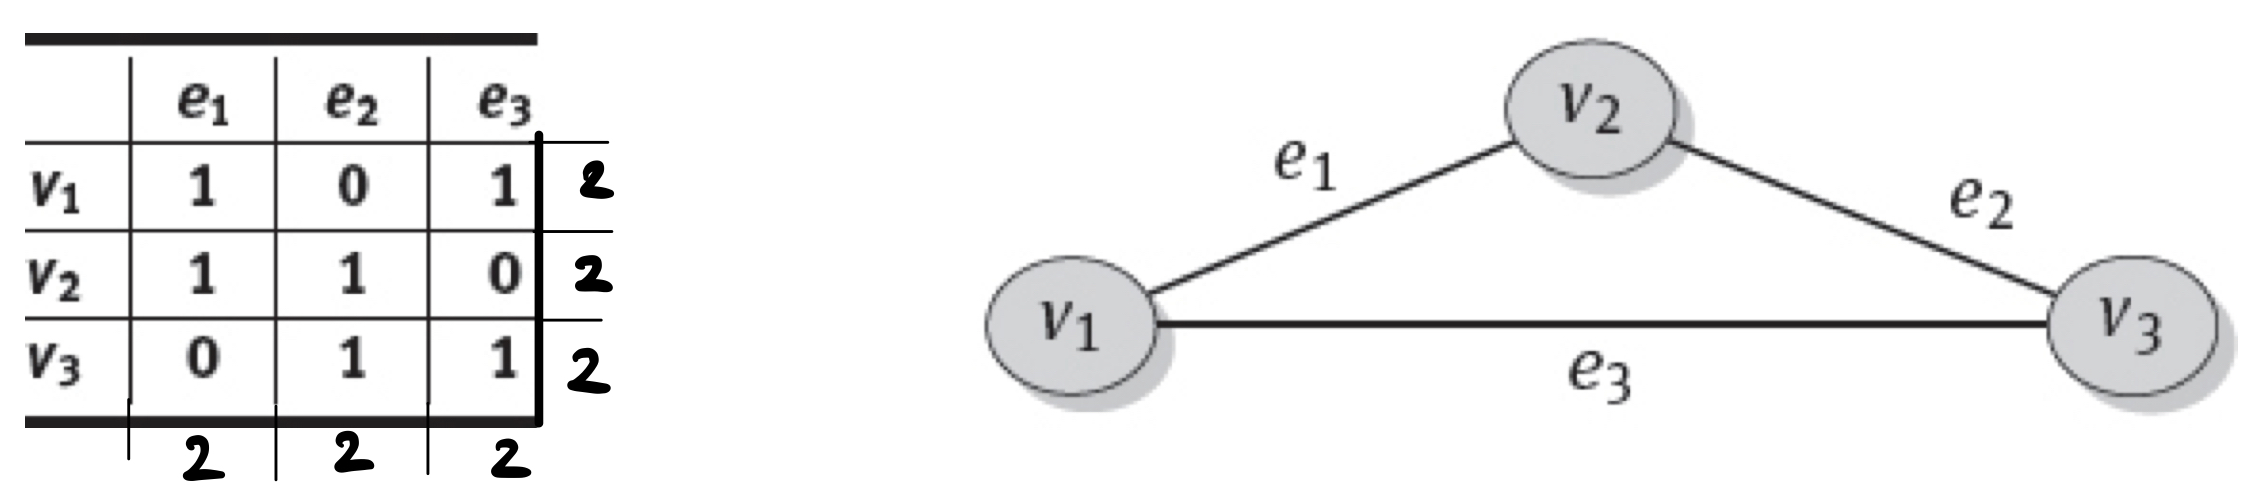
\includegraphics[width=0.7\linewidth]{images/AdvancedDataManagment/graph_databases/inc_matrix_simple_undirected.jpeg}
        \end{figure}
    
    \item \textbf{Simple directed graph}
    \begin{itemize}
        \item For edge \(e_k = (v_i, v_j)\) we write \(-1\) in cell \((v_i, e_k)\) and \(1\) in cell \((v_j, e_k)\)
        \item In case of \textit{loop} \(e_k = \{v_i, v_i\}\) we write \(2\) in the corresponding cell \((v_i, e_k)\)
    \end{itemize}
    
    \begin{figure}[!h]
        \centering
        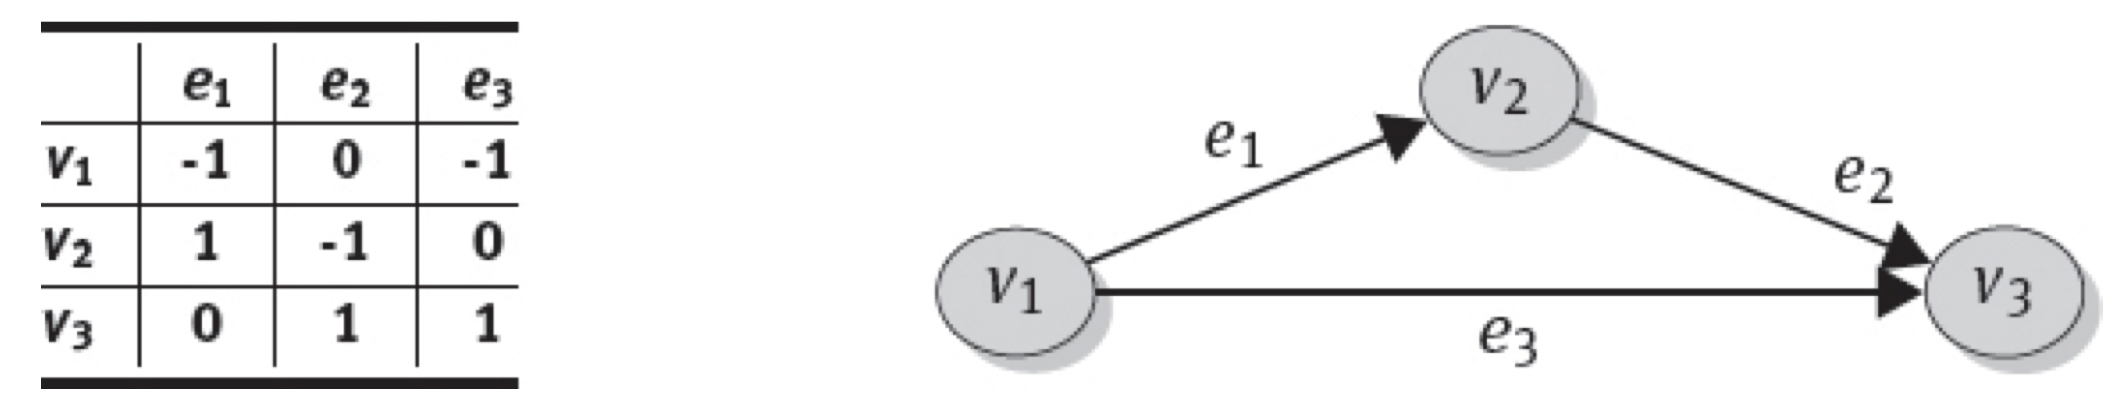
\includegraphics[width=0.7\linewidth]{images/AdvancedDataManagment/graph_databases/inc_matrix_simple_directed.jpeg}
        \end{figure}
    
    \item \textbf{Undirected multigraph}
    \begin{itemize}
        \item If vertices \(v_i\) is connected to edge \(e_j\) we write \(1\) in the corresponding cell \((v_i, e_j)\)
        \item In case of \textit{loop} \(e_j = \{v_i, v_i\}\) we write \(2\) in the corresponding cell \((v_i, e_j)\)
    \end{itemize}
    
    \begin{figure}[!h]
        \centering
        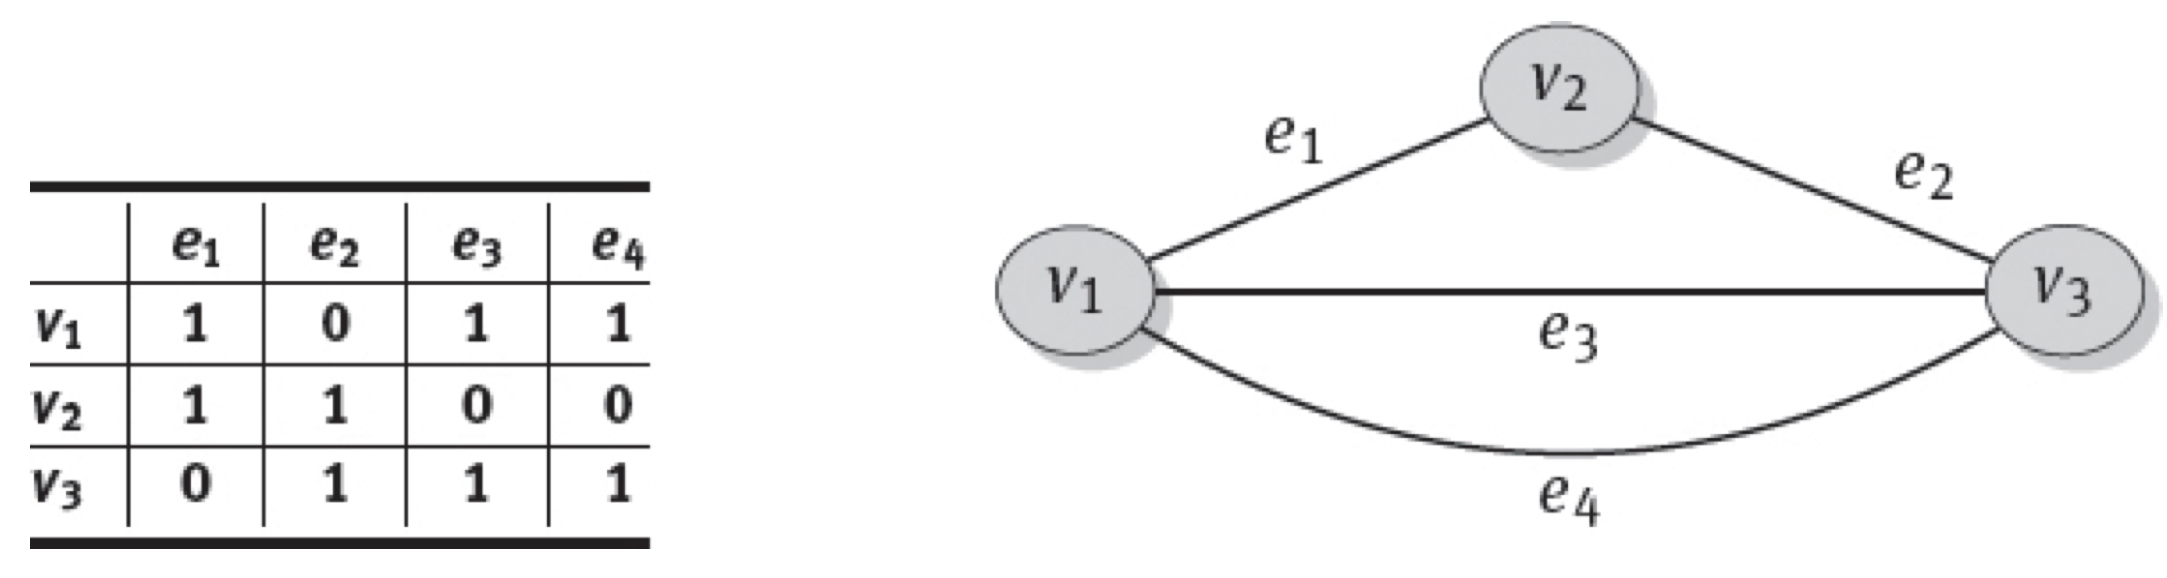
\includegraphics[width=0.7\linewidth]{images/AdvancedDataManagment/graph_databases/inc_matrix_multi_undirected.jpeg}
        \end{figure}
    \newpage
    \item \textbf{Directed multigraph}
    \begin{itemize}
        \item For edge \(e_k = (v_i, v_j)\) we write \(-1\) in cell \((v_i, e_k)\) and \(1\) in cell \((v_j, e_k)\)
        \item In case of \textit{loop} \(e_k = \{v_i, v_i\}\) we write \(2\) in the corresponding cell \((v_i, e_k)\)
    \end{itemize}
    
    \begin{figure}[!h]
        \centering
        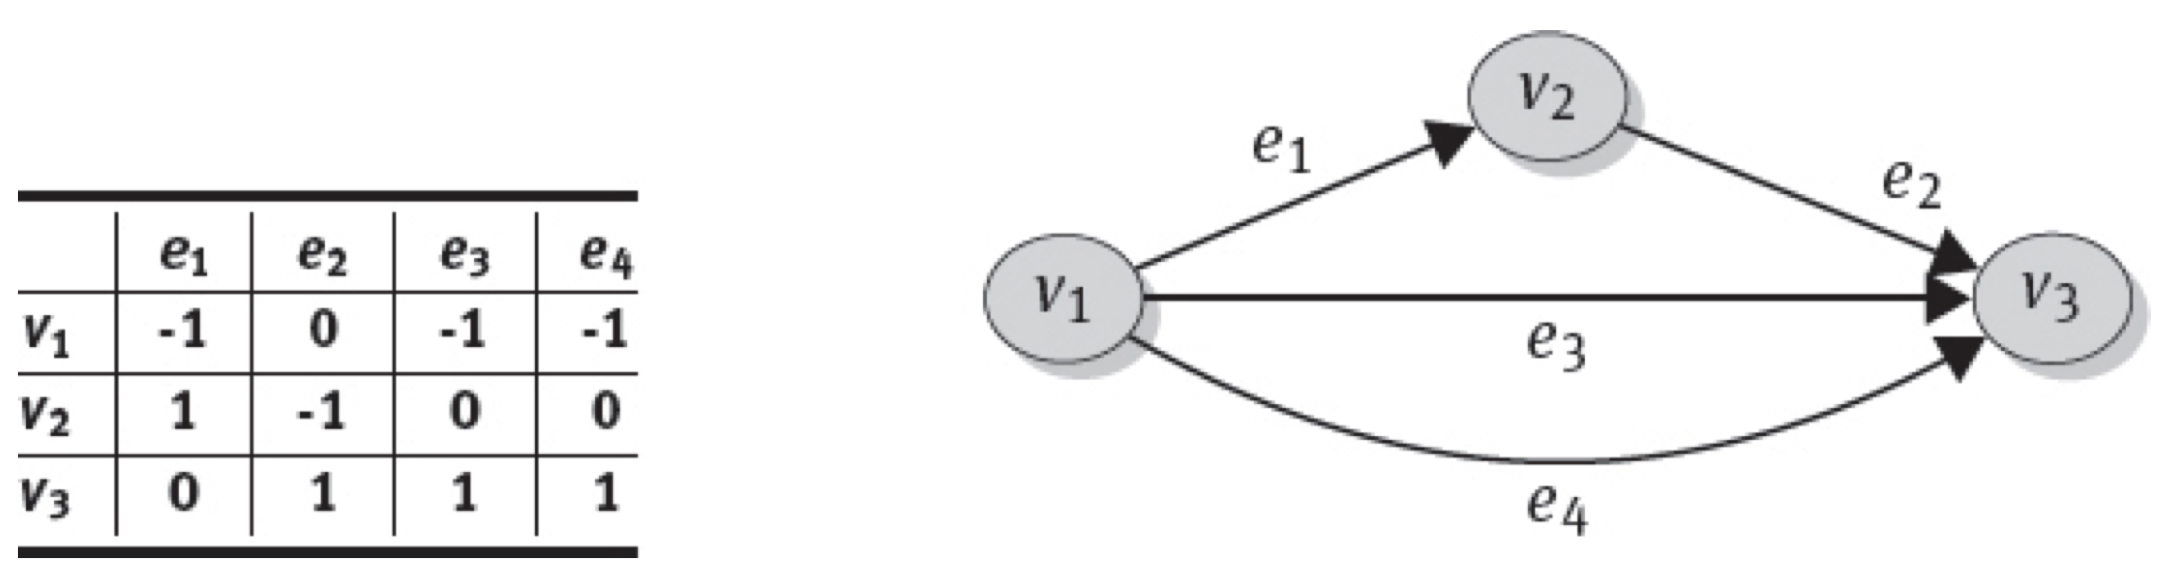
\includegraphics[width=0.7\linewidth]{images/AdvancedDataManagment/graph_databases/inc_matrix_multi_directed.jpeg}
        \end{figure}
    
    
\end{itemize}
\subsubsection{Advantages}
\begin{itemize}
    \item Only existing edges are stored, there is no column with only 0 entries
    \item Hyperedges can be stored
\end{itemize}

\subsubsection{Disadvantages}
\begin{itemize}
    \item Insertions of new vertices and edges are costly, since the addition of a row or a column
    \item Determining all neighbors for one vertex requires scanning the entire row and for each non-zero entry
    \item \(n \times n\) matrices are heavy
    \item Unnecessary information, indeed lots of 0s in the columns 
\end{itemize}

Note that \textbf{checking the existence of an edge} is more involved for the \textit{incidence matrix} than for the adjacency matrix: we have to check whether there is a column with appropriate non-zero entries for the source node’s row and the target node’s row.

\subsection{Adjacent List}
It stores the vertex set \(V\) and for each vertex one stores a \textbf{linked list of neighboring}
\begin{itemize}
    \item \textbf{Simple undirected graph:} each edge is stored in the adjacency list of both its vertices
    \begin{figure}[!h]
        \centering
        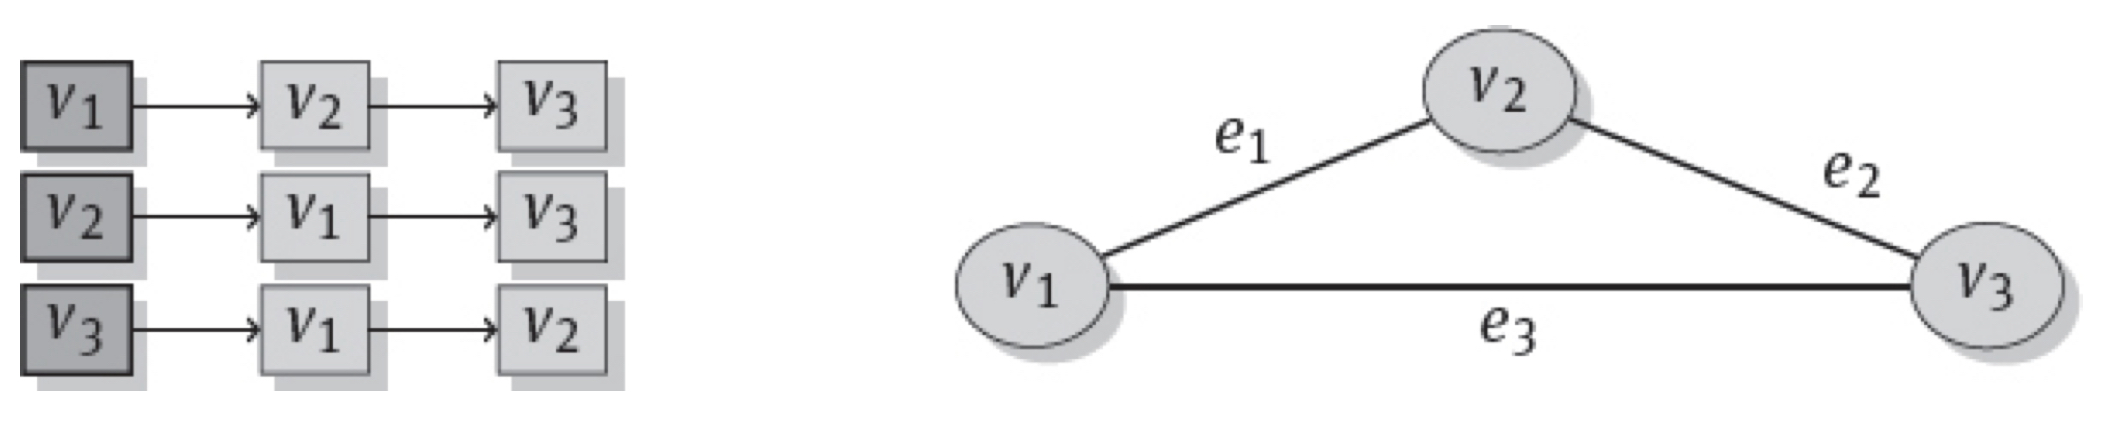
\includegraphics[width=0.7\linewidth]{images/AdvancedDataManagment/graph_databases/adj_list_simple_undirected.jpeg}
        \end{figure}
    \newpage
    \item \textbf{Simple directed graph:} it stores only outgoing edges
    \begin{figure}[!h]
        \centering
        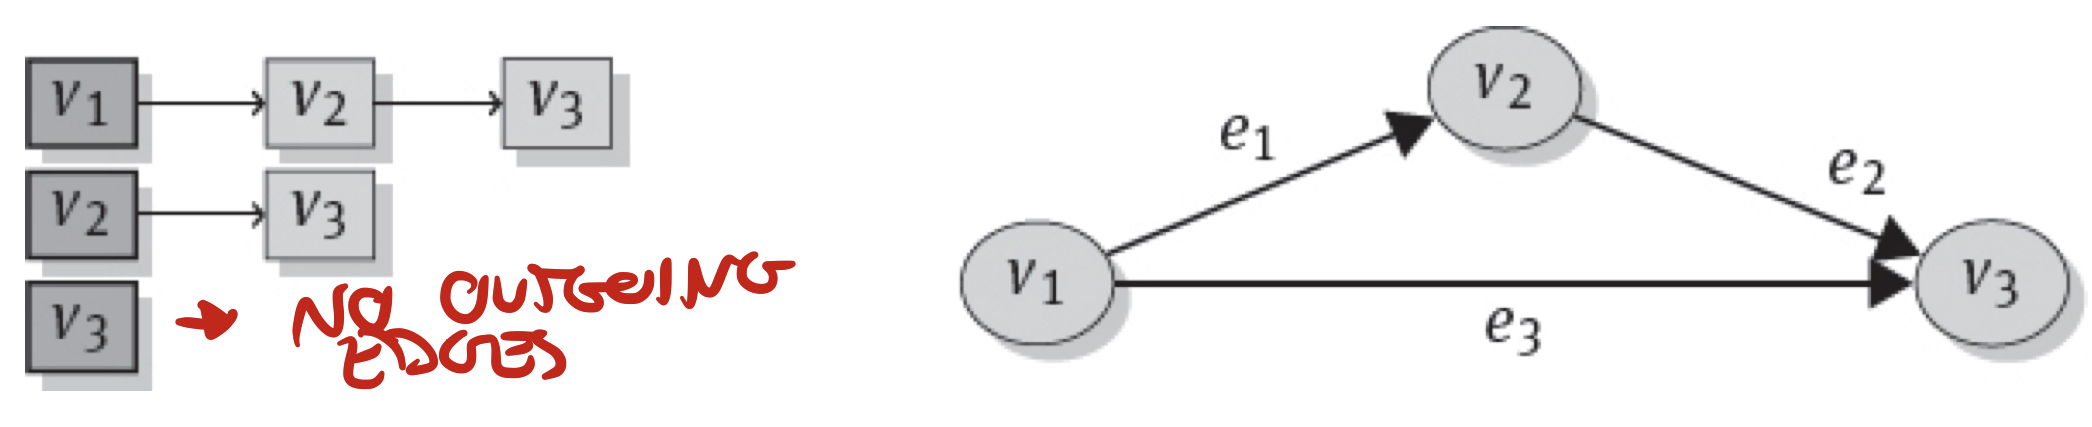
\includegraphics[width=0.7\linewidth]{images/AdvancedDataManagment/graph_databases/adj_list_simple_directed.jpeg}
        \end{figure}
    
    
    \item \textbf{Multigraphs:} in both the directed as well as the undirected case, nodes can occur multiple times in an adjacency list
    \begin{figure}[!h]
        \centering
        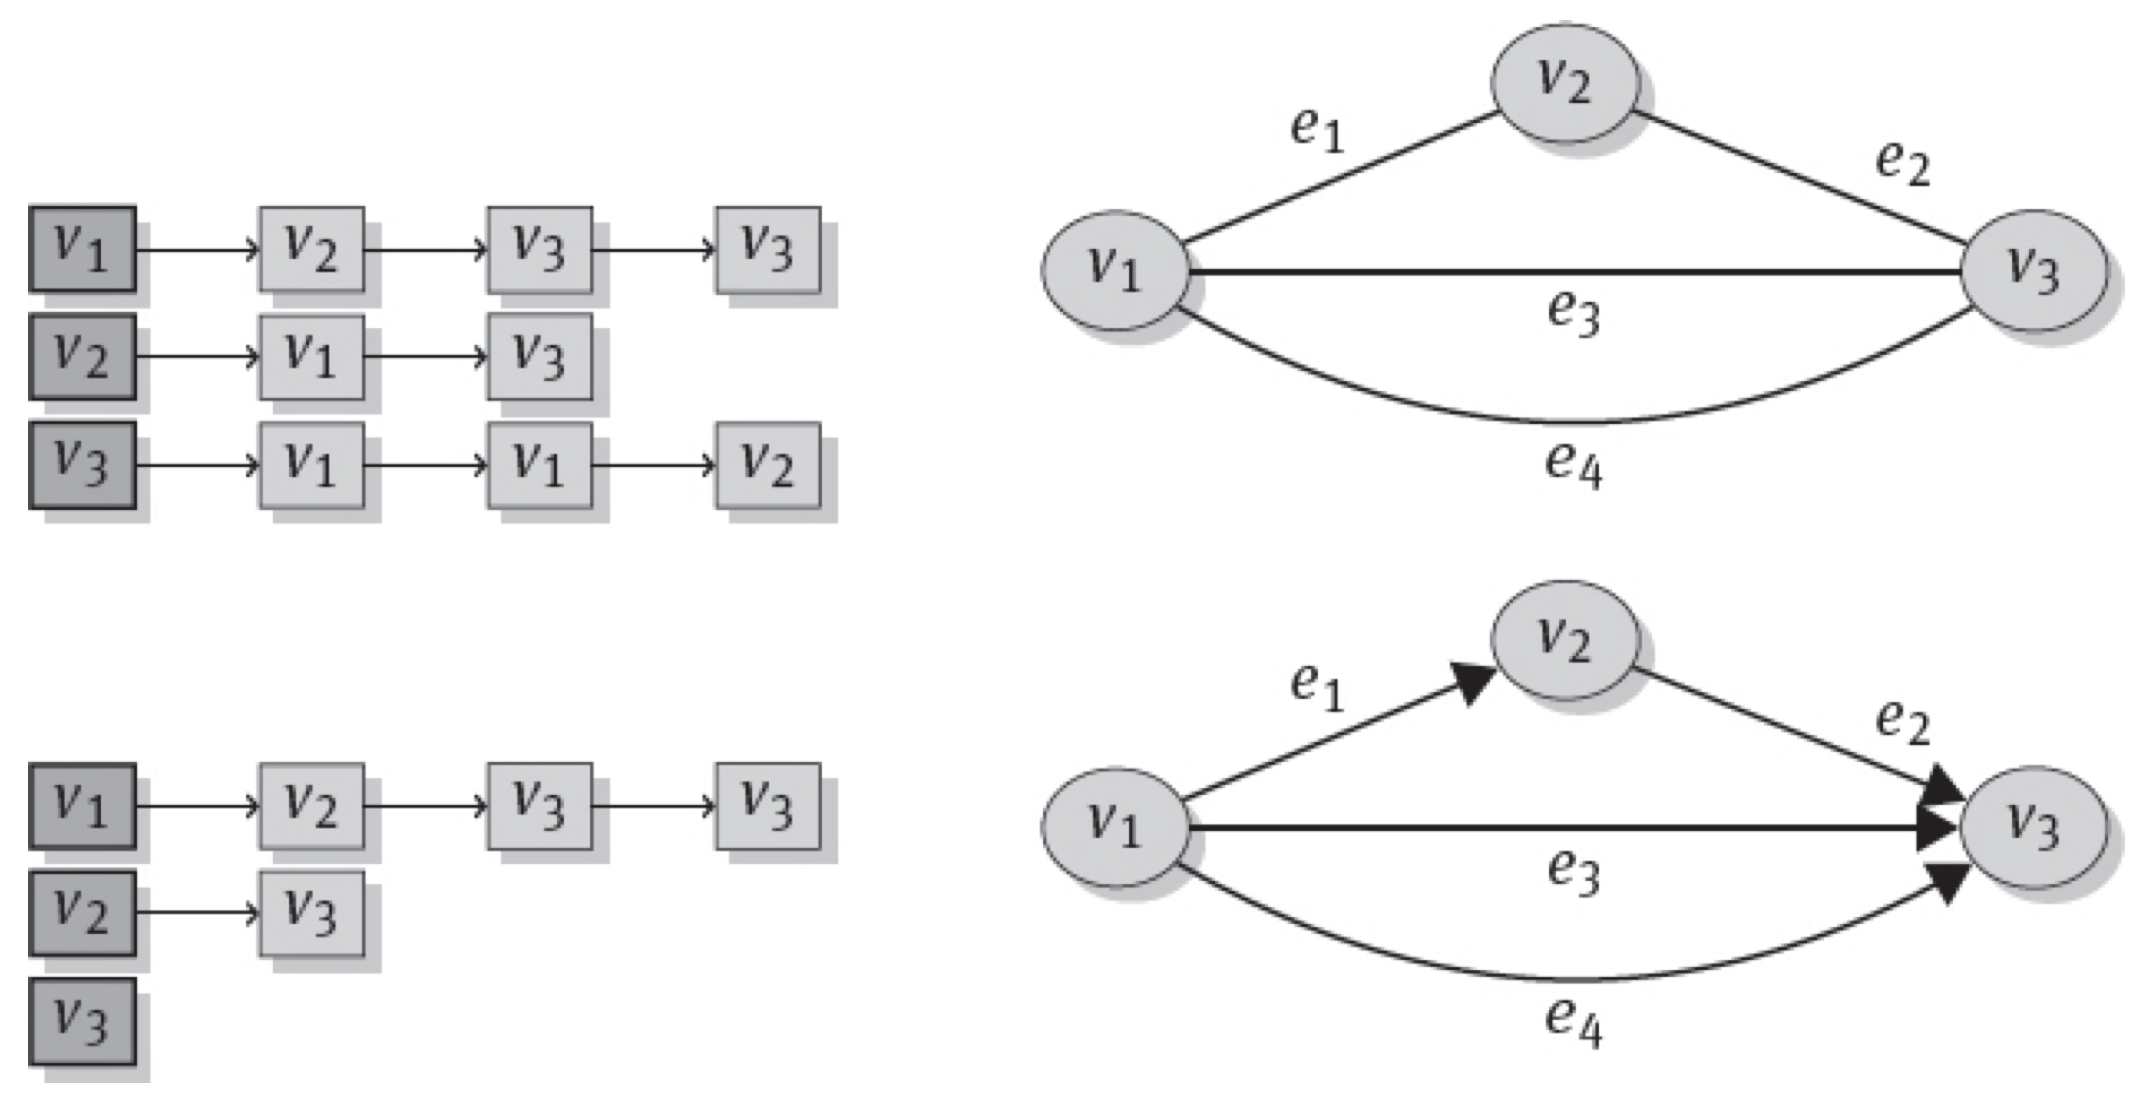
\includegraphics[width=0.7\linewidth]{images/AdvancedDataManagment/graph_databases/adj_list_multi.jpeg}
        \end{figure}
    
\end{itemize}
\subsubsection{Advantages}
\begin{itemize}
    \item Quick insertion of new vertices and edges
    \item Quick lookup of all neighboring vertices
    \item No storage overhead occurs
    \item Hyperedges can be stored
\end{itemize}

\subsubsection{Disadvantages}
\begin{itemize}
    \item Checking existence of a single edge requires a full scan of the adjacency list of the source node
\end{itemize}

\subsection{Incidence List}
With an incidence list, you store the \textbf{vertex set} \(V\) and for each vertex you store a \textbf{linked list of incident edges}
\begin{itemize}
    \item When the edge is \textit{directed} the edge object contains information on its \textbf{source} node and its \textbf{target node}
    \item When the edge is \textit{undirected} no difference is made between source and target nodes
\end{itemize}
\begin{itemize}
    \item \textbf{Simple undirected graph:} each undirected edge is contained in the incidence lists of its two connected nodes
    \begin{figure}[!h]
        \centering
        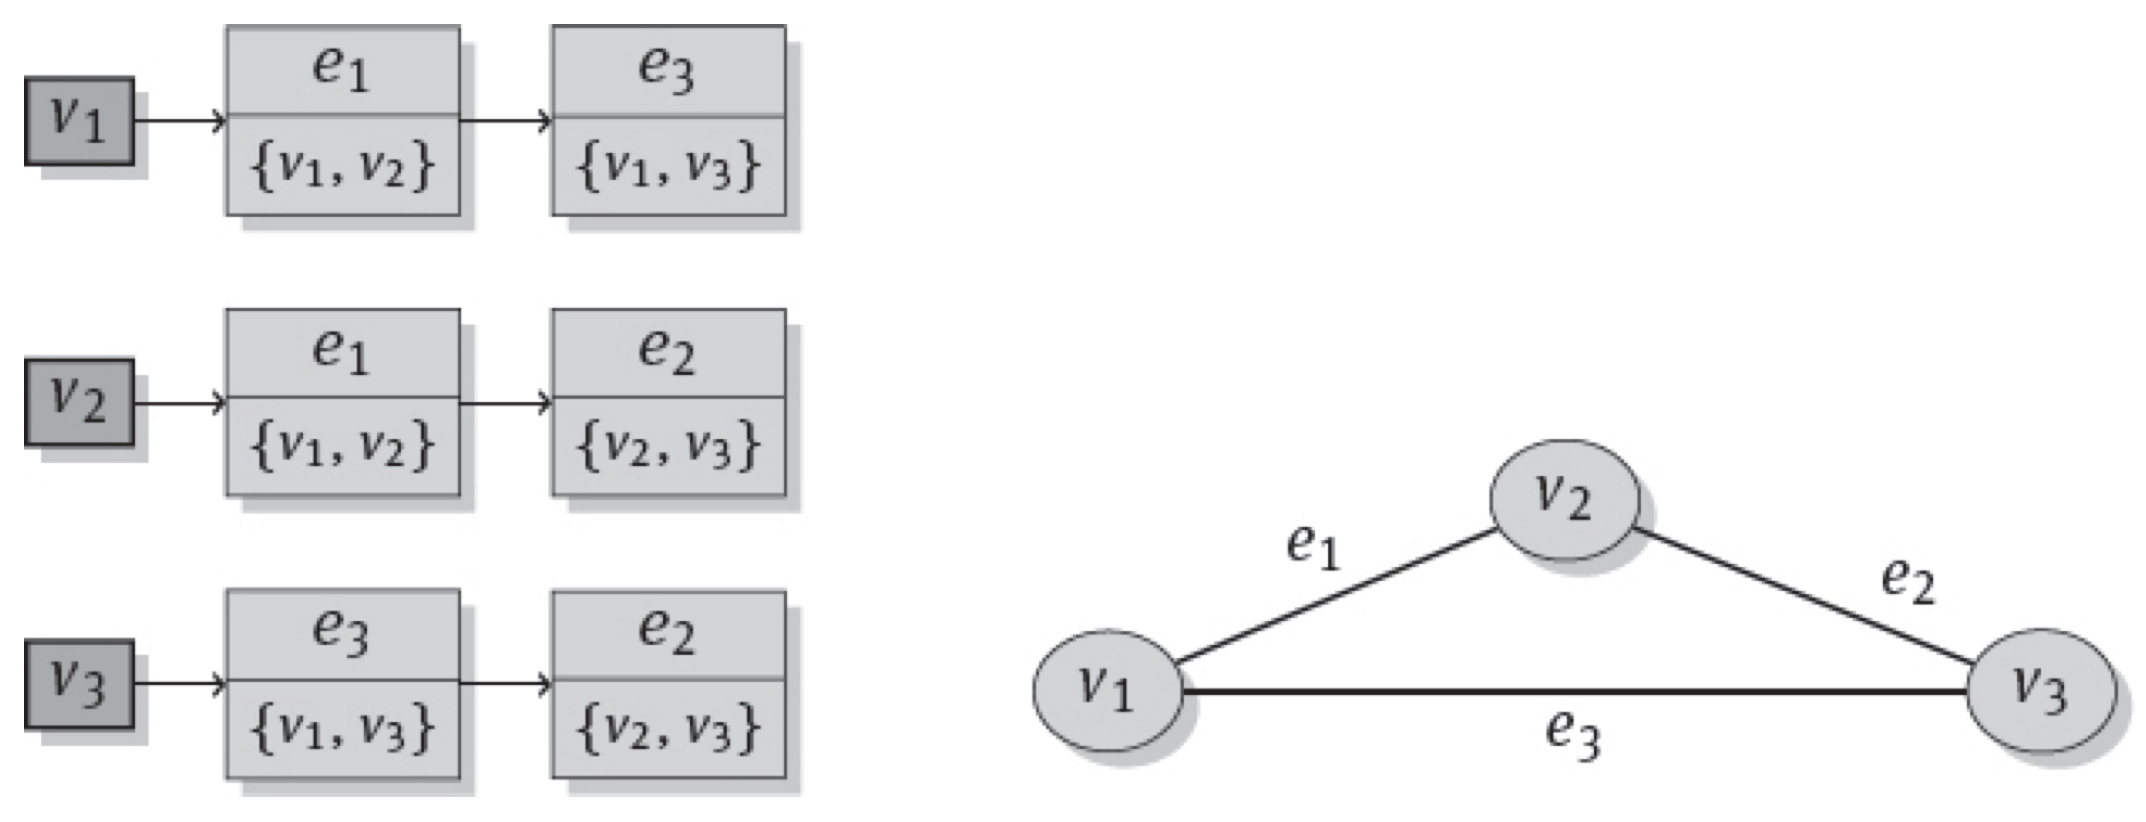
\includegraphics[width=0.7\linewidth]{images/AdvancedDataManagment/graph_databases/inc_list_simple_undirected.jpeg}
        \end{figure}
    
    \item \textbf{Simple directed graph:} it suffices to store only outgoing edges in the incidence list as long as only a forward traversal of the edges is needed. In this case, it is advantageous to store all incident edges in a node’s incidence list to allow for both forward traversal of the outgoing edges and backward traversal of the incoming edges. We could have two incidence list>
    \begin{itemize}
        \item One for the \textbf{outgoing} edges for the forward traversal
        \item One for the \textbf{incoming} edges for the backword traversal
    \end{itemize}
    \begin{figure}[!h]
        \centering
        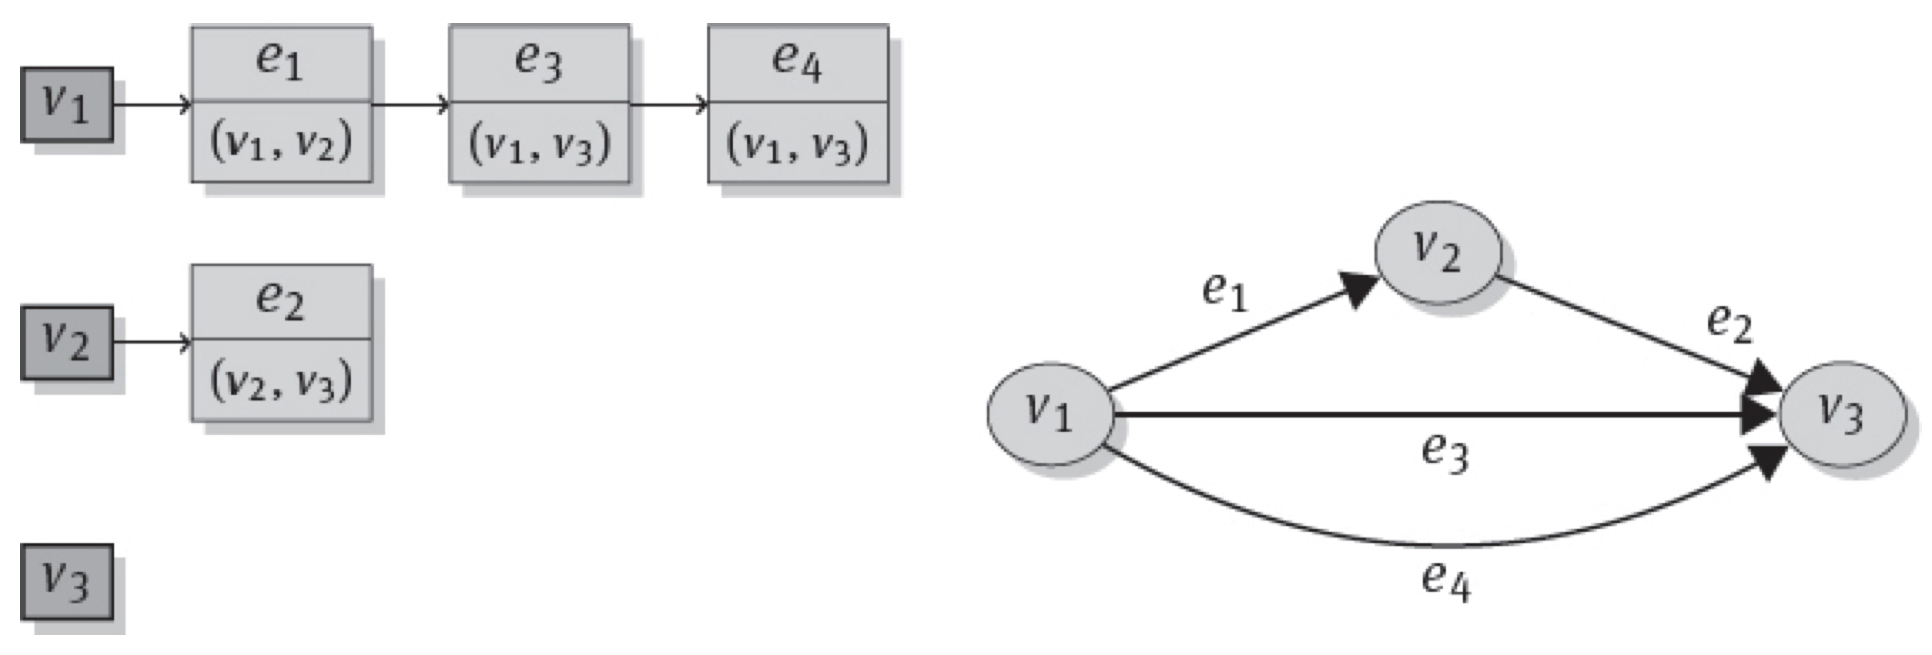
\includegraphics[width=0.7\linewidth]{images/AdvancedDataManagment/graph_databases/inc_list_simple_directed.jpeg}
        \end{figure}
    
    \item \textbf{Multigraphs:} in both directed as well as the undirected case, each edge has its own identity and hence is stored separately.
    \begin{itemize}
        \item For the \textbf{undirected} case each edge contains pointer to the incident nodes
        \begin{figure}[!h]
        \centering
        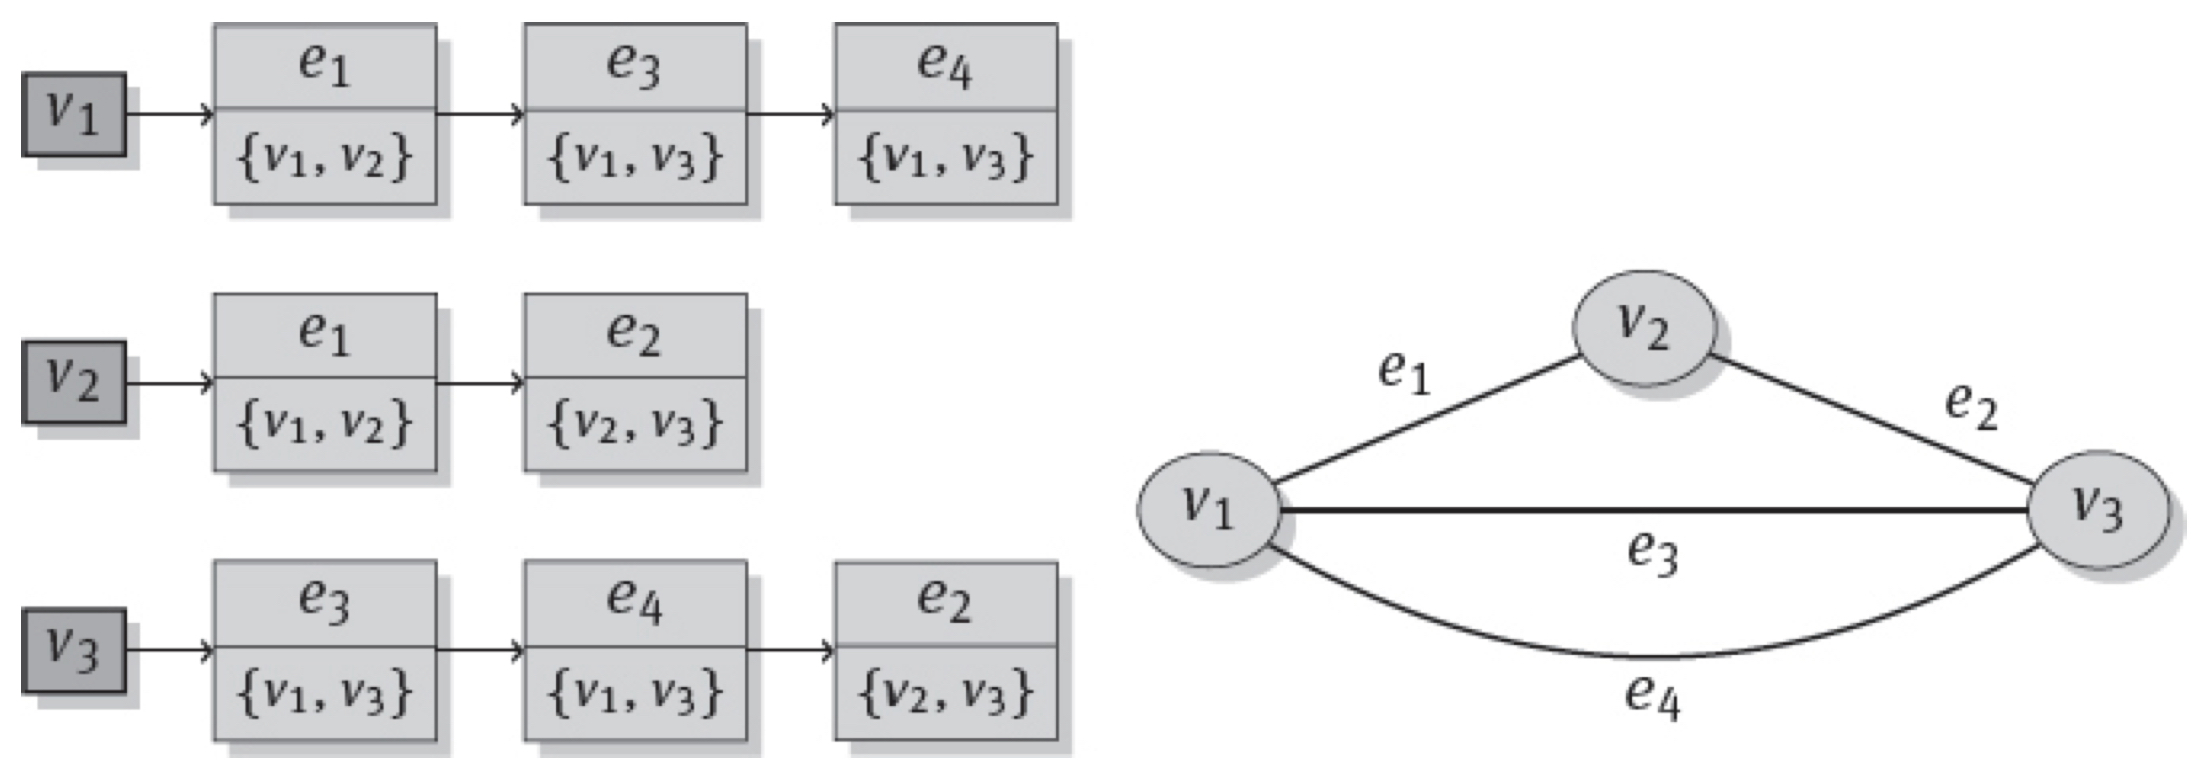
\includegraphics[width=0.7\linewidth]{images/AdvancedDataManagment/graph_databases/inc_list_multi_undirected.jpeg}
        \end{figure}
        \newpage
        \item For the \textbf{directed} case each edge would have a pointer to its source node as well as one pointer to its target node
        \begin{figure}[!h]
        \centering
        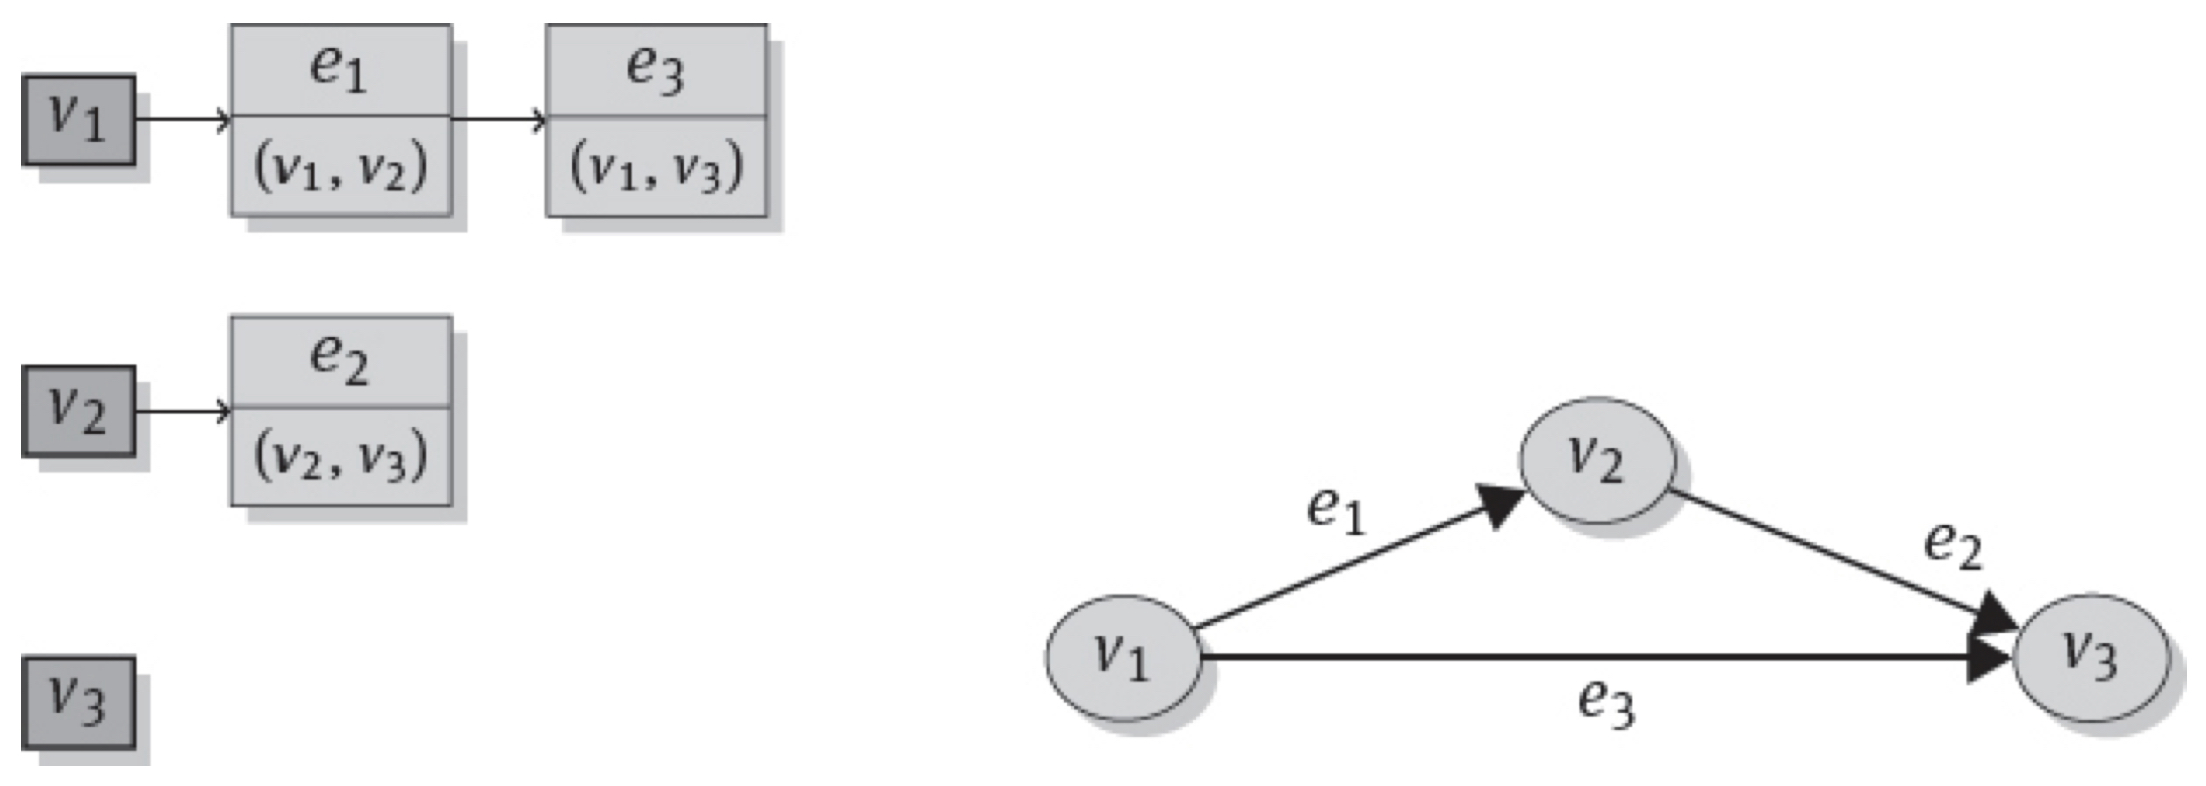
\includegraphics[width=0.7\linewidth]{images/AdvancedDataManagment/graph_databases/inc_list_multi_directed.jpeg}
        \end{figure}
    \end{itemize}
\end{itemize}
In practical implementations, the incidence list would be \textbf{stored inside a node object} as a \textbf{collection of pointers} to incident edge objects – potentially – in the directed case – one collection for incoming and one collection for outgoing edges to allow for both forward and backward traversal.

\section{The Property Graph Model}
\begin{itemize}
    \item The basic storage structure usually is a directed multigraph
    \item We must be able to \textbf{store information} inside the \textit{node} as well as along the \textit{edges}
    \item We must be able to distinguish different kind of nodes and edges. Point achieved by the \textbf{multi-relational} graph where \textbf{types} are introduced for nodes and edges.
    \begin{itemize}
        \item Each node is labeled with the \textbf{node label} that correspond to the node type
        \item Each edge is labeled with the \textbf{edge label} that correspond to the edge type
    \end{itemize}
    \item A type defines \textbf{attributes} for the corresponding nodes and edges. So an attribute definition must contain a name for the attribute and it mus specify a domain of values
    \item Like \textit{name:value} pairs describe \textbf{proprieties} of a node or edge
    \item \textbf{Edge labels} between any two nodes should be \textbf{unique}
    \item Each node has a system-defined \textbf{unique identifier}
\end{itemize}
A propriety graph \(G\) can be defined as \(G = (V, E, L_V, L_E, ID)\):
\begin{itemize}
    \item \(V\) set of \textbf{nodes}
    \item \(E\) set of \textbf{edges}
    \item \(L_V\) set of \textbf{node labels} st to each label \(l \in L_E\) we can assign a set of attribute definitions
    \item \(L_E\) set of \textbf{edge labels} st to each label \(l \in L_E\) we can assign a set of attribute definitions
    \item \(ID\) set of identifiers that can uniquely be assigned to nodes and edges
\end{itemize}
A specific node \(v \in V\) has the following definition: \(v = (id, l, P)\):
\begin{itemize}
    \item \(id \in ID\)
    \item \(l \in L_V\)
    \item \(P\) is a set of proprieties, st each \textbf{propriety} \(p \in P\) is a \textit{name:value}-pair st:
    \begin{itemize}
        \item The \textit{name} correspond to an attribute name defined by the node type
        \item The \textit{value} is a valid value taken from the teh attribute domain
    \end{itemize}
\end{itemize}
Similarly an edge \(e \in E\) is defined like so \(e = (id, l', P, source, target)\):
\begin{itemize}
    \item \(l'\) is an edge label from \(L_E\)
    \item The proprieties in \(P\) correspond to an attribute definitions of this edge type
\end{itemize}

\subsubsection{Example}
\begin{figure}[!h]
        \centering
        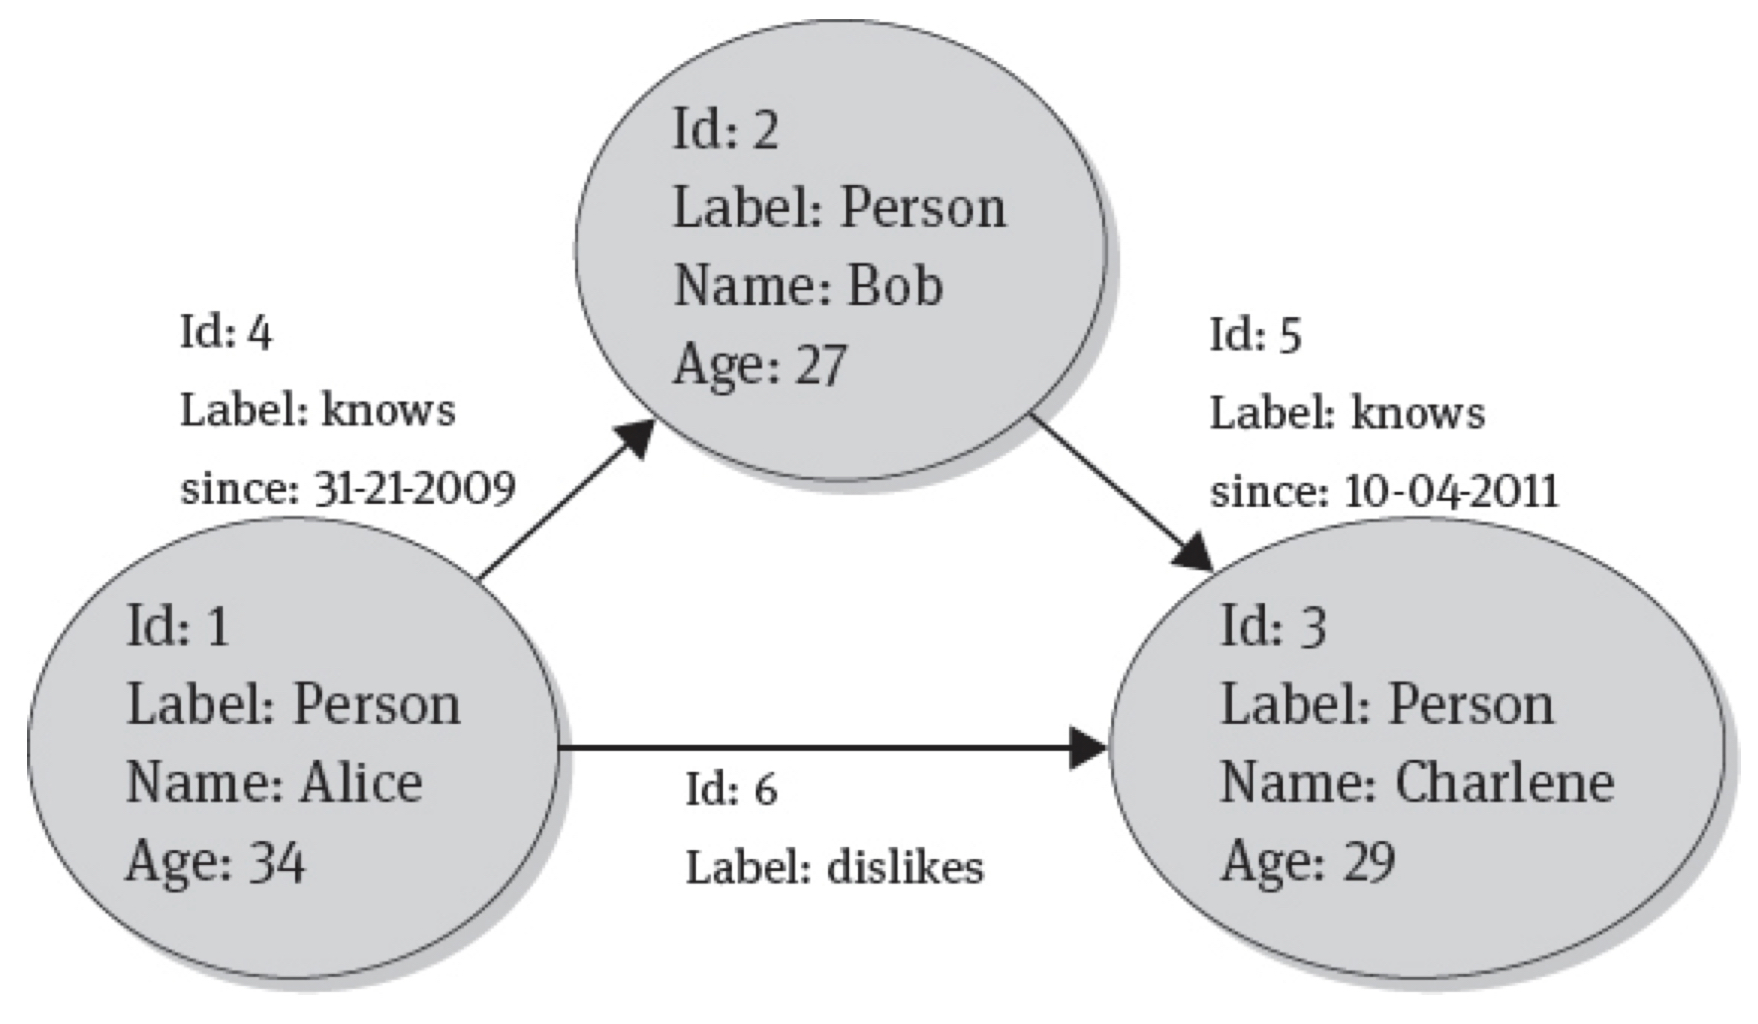
\includegraphics[width=0.7\linewidth]{images/AdvancedDataManagment/graph_databases/propriety_graph_example.jpeg}
        \caption{A property graph for a social network}
        \end{figure}
\begin{itemize}
    \item The node set is \(V = \{v_1, v_2, v_3\}\)
    \item The edge set is \(E = \{e_1, e_2, e_3\}\)
    \item The node labels are \(L_V = \{Person\}\)
    \item The node type definitions are \(t_{Person} = \{Person, A_{Person}\}\) where the attribute definitions are \textit{APerson} = \textit{\{(Name, String), (Age, Integer)\}}
    \item The edge labels are \(L_E = \{knows, dislikes\}\)
    \item The edge type definitions are \(t_{knows} = \{knows, A_{knows}, \{Person\}, \{Person\}\}\) and \(t_{dislikes} = \{dislikes, \emptyset, \{Person\}, \{Person\}\}\), where \textit{Aknows = \{(since, Date)\}}
\end{itemize}
The specification of nodes and edges are the following:
\begin{itemize}
    \item \(v_1 =\) \textit{\{1, Person, \{Name: Alice, Age: 34\}\}}
    \item \(v_2 =\) \textit{\{2, Person, \{Name: Bob, Age: 27\}\}}
    \item \(v_3 =\) \textit{\{3, Person, \{Name: Charlene, Age: 29\}\}}
    \item \(e_1 =\) \textit{\{4, knows, \{since: 31-21-2009\}, 1, 2\}}
    \item \(e_2 =\) \textit{\{5, knows, \{since: 10-04-2011\}, 2, 3\}}
    \item \(e_3 =\) \textit{\{6, dislikes, ;, 1, 3\}}
\end{itemize}

In addition we specify an additional requirement: \textbf{there may never be two edges with the same label between two nodes.} Like the following example
\begin{figure}[!h]
    \centering
    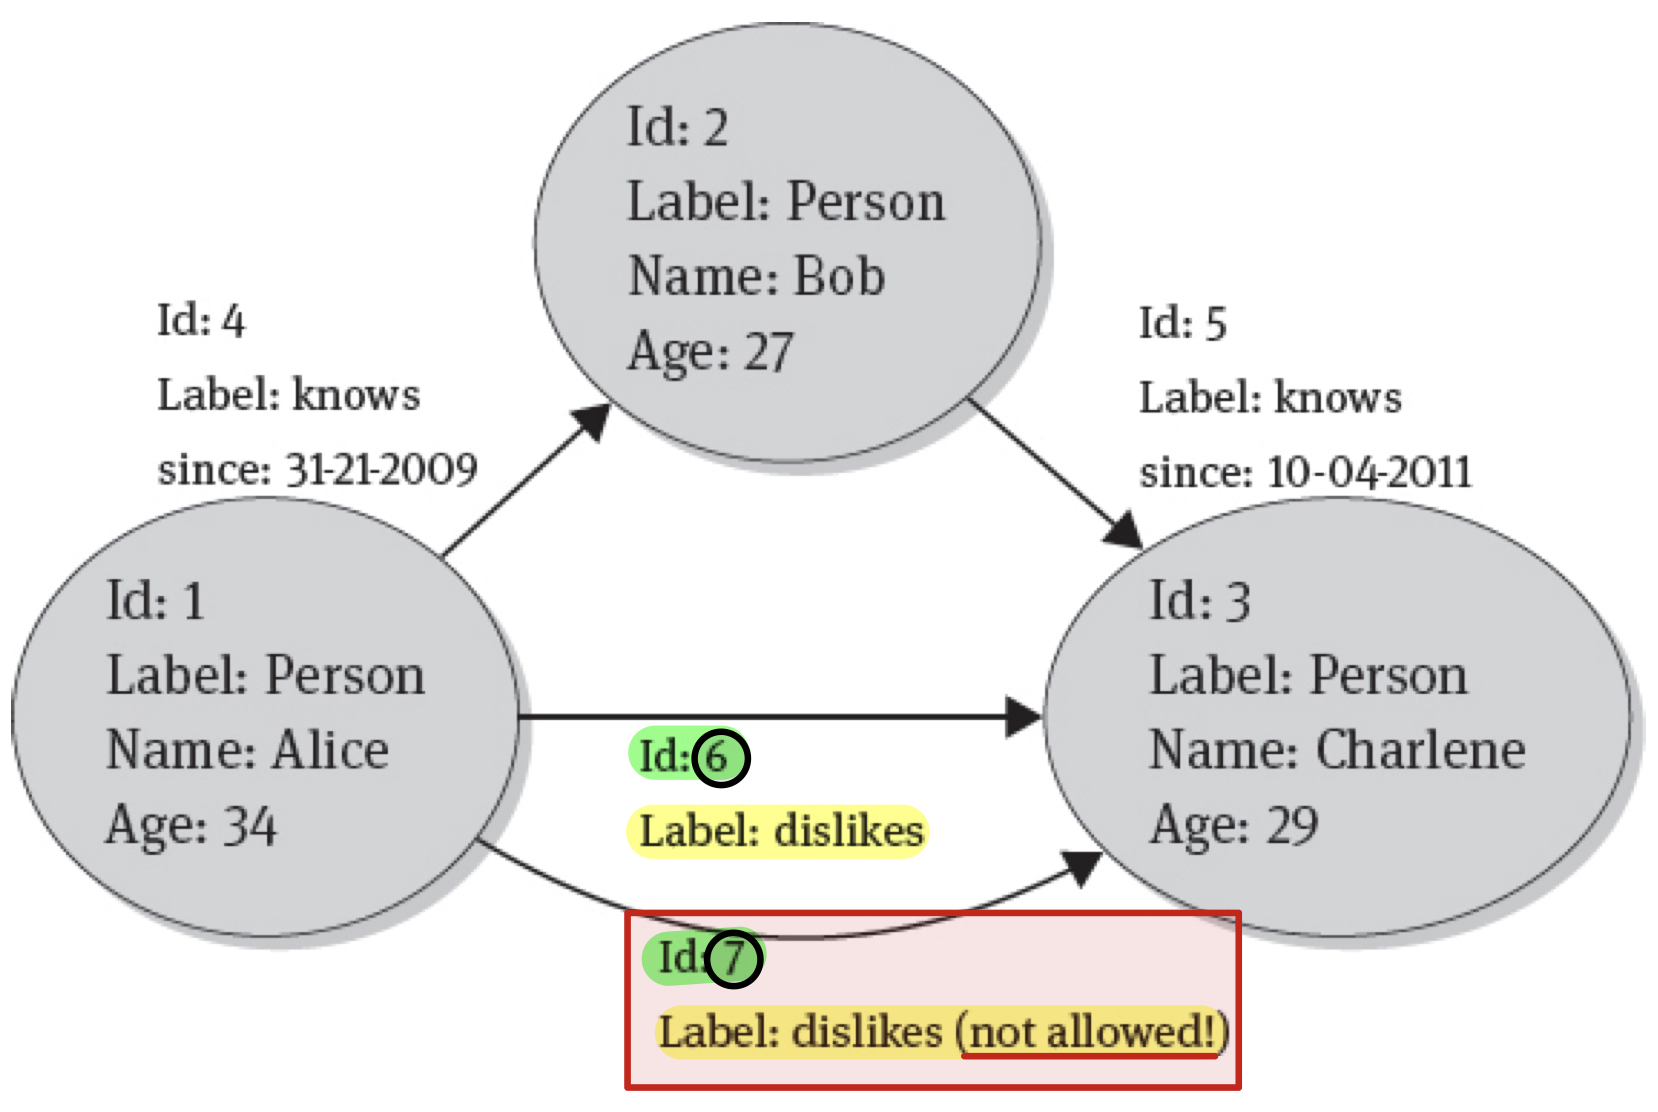
\includegraphics[width=0.7\linewidth]{images/AdvancedDataManagment/graph_databases/violation_example.jpeg}
    \caption{Violation of uniqueness of edge labels}
\end{figure}